\definecolor{rewriteGray}{HTML}{A0A0A0}
\definecolor{rewriteBlue}{HTML}{4C78A8}
\definecolor{rewriteOrange}{HTML}{F28E2B}
\definecolor{rewriteGreen}{HTML}{59A14F}

\tikzset{
  rewrite cell/.style={draw=black!75,minimum width=.66cm,
    minimum height=.50cm,inner sep=0pt,font=\footnotesize},
  rewrite old/.style={rewrite cell,fill=rewriteGray!20},
  rewrite new/.style={rewrite cell,draw=rewriteBlue!90!black,
    fill=rewriteBlue!14},
  rewrite min/.style={rewrite cell,draw=rewriteOrange!90!black,
    very thick,fill=rewriteOrange!18},
  rewrite out/.style={rewrite cell,draw=rewriteGreen!80!black,
    very thick,fill=rewriteGreen!16},
  rewrite box/.style={draw=black!75,align=center,inner sep=4pt,
    minimum height=.78cm,font=\footnotesize},
  rewrite flow/.style={-{Latex[length=1.8mm]},thick},
  rewrite note/.style={draw=black!65,align=left,inner sep=5pt,
    font=\footnotesize}
}

% This chapter keeps figures, tables, and algorithms beside their discussion.
% Avoid stretching the surrounding paragraphs when a non-floating object moves
% to the next page because it does not fit in the remaining space.
\raggedbottom

\section{From every base to a sparse, comparable sketch}
\label{sec:minimizers-role}

The first computational stage of the BioSeqDB aligner needs to compute
\(\operatorname{Seed}(X)\).
A target seed becomes a key in an index and then query seed is looked
up in that index, and each occurrence (so shared seed between query and target) becomes an anchor for the
chaining stage described in Section~\ref{sec:chaining-purpose}. 

We expect the seed set to be sparse enough to reduce index and lookup costs, but dense enough that related sequences have common seeds.
As described before minimap2 and BioseqDB operate on minimizers. I didn't specifically added support for "true" cannonical minimizers in a sense that I 
adhered to the minimap2 approach i.e taking minimum of hashes of k-mer and its reverse complement.

Formally, let $S=s_0s_1\ldots s_{n-1}$ be a nucleotide sequence. The $k$-mer beginning
at zero-based position $i$ is
\[
  K_i=S[i,i+k).
\]
For DNA, the forward and reverse-complement encodings are
\[
  F_i=\operatorname{enc}(K_i),
  \qquad
  R_i=\operatorname{enc}(\overline{K_i}).
\]
A canonical $k$-mer uses the same key on both strands. A common choice is
\[
  C_i=\min(F_i,R_i),
  \qquad
  z_i=\mathbf{1}[R_i<F_i],
\]
where $z_i$ records the selected strand. Applying a hash function $H$ gives a
candidate
\[
  x_i=(h_i,p_i,z_i),
  \qquad
  h_i=H(C_i).
\]
The position $p_i$ may denote the first or final base of $K_i$. BioSeqDB's
minimap-compatible schemes use the final base because that is the convention
used by minimap2~\cite{minimap2_paper}.

For a window of $w$ consecutive candidates,
\[
  W_j=(x_j,x_{j+1},\ldots,x_{j+w-1}),
  \qquad
  m_j=\min_{x\in W_j}h(x).
\]
The expected density is theoretically $2/(w+1)$ minimizers per
candidate position.~\cite{shur_minimum_density_2025}, however practically it might vary. Minimap2 for example uses 
HPC (homopolymer-compressed) encoding which means that repeated letters are compressed so we don't extract repeated minimizers for sections that are larege single-letter segments.
In BioseqDB I do not support HPC compression.

There are also other practical and theoretical consideratiosn affecting minimizer extraction like different formulations of hashing functions or heuristics to avoid having very low minimizer density in 
specific repeated regions, but I won't go into very specific details.

Figure~\ref{fig:minimizer-walkthrough} shows what happens to one $k$-mer through hashing,
selection of window that its belongs to and dedupliction of hashes.

\begin{figure}[H]
\centering
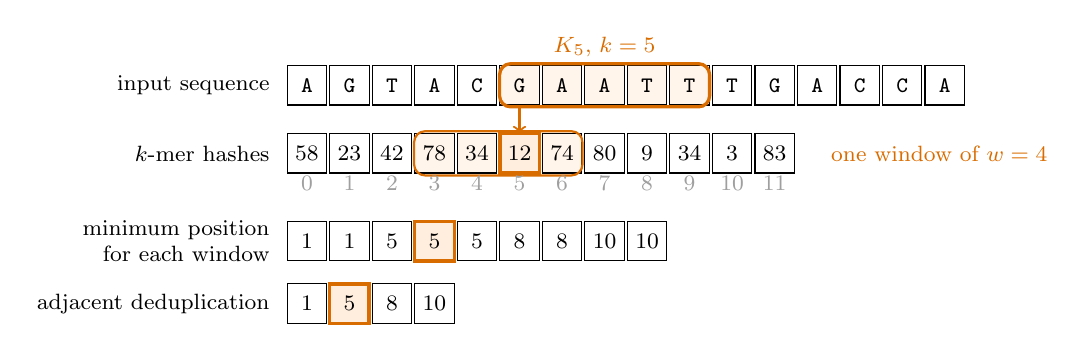
\begin{tikzpicture}[
  x=.54cm,
  y=.72cm,
  font=\footnotesize,
  cell/.style={draw,minimum width=.50cm,minimum height=.50cm,inner sep=0pt},
  tracked/.style={draw=orange!85!black,very thick,fill=orange!13,
                  minimum width=.50cm,minimum height=.50cm,inner sep=0pt},
  context/.style={draw,fill=orange!8,minimum width=.50cm,
                  minimum height=.50cm,inner sep=0pt}
]
  \node[anchor=east] at (4.35,4.10) {input sequence};
  \foreach \i/\v in {0/A,1/G,2/T,3/A,4/C,5/G,6/A,7/A,8/T,9/T,10/T,11/G,12/A,13/C,14/C,15/A}
    \node[cell] (s\i) at (5+\i,4.10) {\texttt{\v}};
  \foreach \i/\v in {5/G,6/A,7/A,8/T,9/T}
    \node[context] at (5+\i,4.10) {\texttt{\v}};
  \draw[orange!85!black,very thick,rounded corners]
    (9.53,3.72) rectangle (14.47,4.48);
  \node[orange!85!black] at (12,4.78) {$K_5$, $k=5$};

  \node[anchor=east] at (4.35,2.90) {$k$-mer hashes};
  \foreach \i/\v in {0/58,1/23,2/42,3/78,4/34,5/12,6/74,7/80,8/9,9/34,10/3,11/83}
    \node[cell] (h\i) at (5+\i,2.90) {\v};
  \foreach \i/\v in {3/78,4/34,6/74}
    \node[context] at (5+\i,2.90) {\v};
  \node[tracked] at (10,2.90) {12};
  \draw[orange!85!black,thick,rounded corners]
    (7.52,2.51) rectangle (11.48,3.29);
  \node[anchor=west,orange!85!black] at (17.10,2.90)
    {one window of $w=4$};
  \foreach \i in {0,...,11}
    \node[gray!75] at (5+\i,2.37) {\i};

  \node[anchor=east,align=right] at (4.35,1.35)
    {minimum position\\for each window};
  \foreach \i/\v in {0/1,1/1,2/5,3/5,4/5,5/8,6/8,7/10,8/10}
    \node[cell] at (5+\i,1.35) {\v};
  \node[tracked] at (8,1.35) {5};

  \node[anchor=east] at (4.35,.25) {adjacent deduplication};
  \foreach \i/\v in {0/1,1/5,2/8,3/10}
    \node[cell] at (5+\i,.25) {\v};
  \node[tracked] at (6,.25) {5};
  \draw[->,thick,orange!85!black] (s5.south) to[out=-90,in=90] (h5.north);
\end{tikzpicture}
\caption{Minimizer extraction for $k=5$ and $w=4$ with illustrative hashes.}
\label{fig:minimizer-walkthrough}
\end{figure}

The hashing function can affect heavily minimizer desnity:
\begin{figure}[H]
\centering
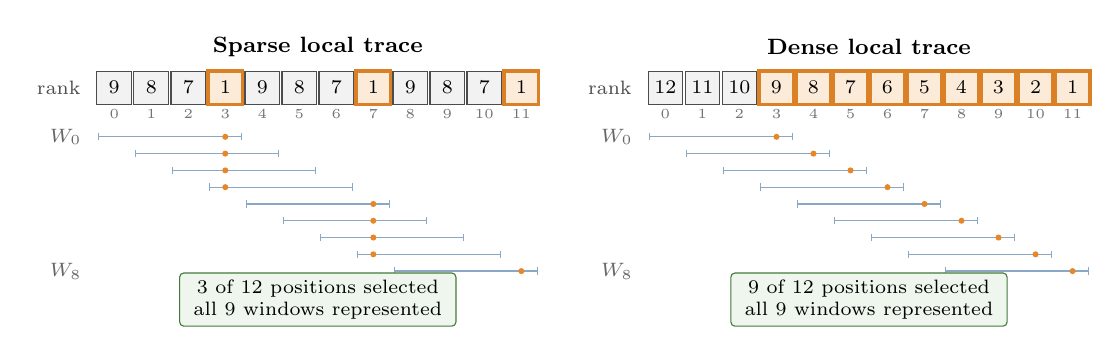
\begin{tikzpicture}[
  x=.47cm,
  y=.26cm,
  font=\scriptsize,
  density cell/.style={
    draw=black!70,
    fill=rewriteGray!14,
    minimum width=.44cm,
    minimum height=.42cm,
    inner sep=0pt
  },
  density selected/.style={
    density cell,
    draw=rewriteOrange!90!black,
    fill=rewriteOrange!18,
    very thick
  },
  density window/.style={
    draw=rewriteBlue!65,
    line width=.45pt
  },
  density count/.style={
    draw=rewriteGreen!75!black,
    fill=rewriteGreen!10,
    rounded corners=1.5pt,
    align=center,
    inner xsep=5pt,
    inner ysep=2.5pt
  }
]
  \begin{scope}
    \node[font=\footnotesize\bfseries] at (5.5,2.0)
      {Sparse local trace};
    \node[anchor=east,text=black!70] at (-.65,0) {rank};

    \foreach \i/\v in {
      0/9,1/8,2/7,3/1,
      4/9,5/8,6/7,7/1,
      8/9,9/8,10/7,11/1
    } {
      \node[density cell] at (\i,0) {\v};
      \node[font=\tiny,text=black!55] at (\i,-1.30) {\i};
    }
    \foreach \i in {3,7,11}
      \node[density selected] at (\i,0) {1};

    \foreach \j in {0,...,8} {
      \pgfmathsetmacro{\wy}{-2.40-.82*\j}
      \pgfmathtruncatemacro{\p}{4*int(\j/4)+3}
      \draw[density window]
        ({\j-.43},\wy) -- ({\j+3+.43},\wy);
      \draw[density window]
        ({\j-.43},{\wy-.18}) -- ({\j-.43},{\wy+.18});
      \draw[density window]
        ({\j+3+.43},{\wy-.18}) -- ({\j+3+.43},{\wy+.18});
      \fill[rewriteOrange!95!black]
        (\p,\wy) circle[radius=1.1pt];
    }

    \node[anchor=east,text=black!60] at (-.62,-2.40) {$W_0$};
    \node[anchor=east,text=black!60]
      at (-.62,{-2.40-.82*8}) {$W_8$};

    \node[density count] at (5.5,-10.35)
      {3 of 12 positions selected\\all 9 windows represented};
  \end{scope}

  \begin{scope}[xshift=7.0cm]
    \node[font=\footnotesize\bfseries] at (5.5,2.0)
      {Dense local trace};
    \node[anchor=east,text=black!70] at (-.65,0) {rank};

    \foreach \i/\v in {
      0/12,1/11,2/10,3/9,4/8,5/7,
      6/6,7/5,8/4,9/3,10/2,11/1
    } {
      \node[density cell] at (\i,0) {\v};
      \node[font=\tiny,text=black!55] at (\i,-1.30) {\i};
    }
    \foreach \i/\v in {
      3/9,4/8,5/7,6/6,7/5,8/4,9/3,10/2,11/1
    }
      \node[density selected] at (\i,0) {\v};

    \foreach \j in {0,...,8} {
      \pgfmathsetmacro{\wy}{-2.40-.82*\j}
      \pgfmathtruncatemacro{\p}{\j+3}
      \draw[density window]
        ({\j-.43},\wy) -- ({\j+3+.43},\wy);
      \draw[density window]
        ({\j-.43},{\wy-.18}) -- ({\j-.43},{\wy+.18});
      \draw[density window]
        ({\j+3+.43},{\wy-.18}) -- ({\j+3+.43},{\wy+.18});
      \fill[rewriteOrange!95!black]
        (\p,\wy) circle[radius=1.1pt];
    }

    \node[anchor=east,text=black!60] at (-.62,-2.40) {$W_0$};
    \node[anchor=east,text=black!60]
      at (-.62,{-2.40-.82*8}) {$W_8$};

    \node[density count] at (5.5,-10.35)
      {9 of 12 positions selected\\all 9 windows represented};
  \end{scope}
\end{tikzpicture}
\caption{Two minimizer traces for \(w=4\). Thin brackets mark candidate
windows, and orange dots mark their selected minima. The left trace reuses
positions 3 and 7. The right trace selects a new position after each slide. Everything depends on numeric properties of used hashing scheme}
\label{fig:minimizer-density-traces}
\end{figure}

I wanted to emphasize that the topic of seed-and-extend is largely based on measuring practical stochastic properties of minimizers distribution and properties and in BioseqDB I only focus
on the simplest approaches where in most cases I use the same hashing scheme as minimap2 to guarantee almost exact sensitivity and in one case discussed later incorporate use of rolling hash (nthash).

Figure~\ref{fig:seed-hash-table} uses fixed four-base seeds on both sides. The
symbols $h_1$, $h_2$, and $h_3$ are some computed hashes. The picture shows that in general we want to build one 
hash table, compare query to the hashes in the hash table and always filter out the most occuring hashes (as this means that this hash does not ultimately distinguish the part that we maching and will 
cause lots of false positives not contributing to the final result)

\begin{figure}[H]
\centering
\begin{tikzpicture}[
  x=.88cm,
  y=.82cm,
  font=\footnotesize,
  >=Latex,
  stage/.style={draw,rounded corners,fill=blue!8,align=center,
                minimum height=.72cm},
  seq/.style={draw=orange!75!black,rounded corners,fill=orange!8,
              align=center,minimum height=.72cm},
  index/.style={draw,very thick,rounded corners,fill=yellow!14,
                align=left,inner sep=5pt},
  output/.style={draw=ForestGreen!70!black,rounded corners,
                 fill=green!7,align=left,inner sep=5pt}
]
  \node[font=\small\bfseries] at (3.1,4.55) {Build the reference index};
  \node[seq,minimum width=5.7cm] (ref) at (3.1,3.65)
    {reference: \texttt{GCTATTACCTTAATGTGATGGAC}};
  \node[stage,minimum width=5.7cm] (rseed) at (3.1,2.55)
    {extract $k=4$: \texttt{GCTA}@0, \texttt{TTAA}@9,
     \texttt{ATGT}@12};
  \node[stage,minimum width=5.7cm] (rhash) at (3.1,1.45)
    {hash: $h_1$, $h_2$, $h_3$};

  \node[index] (table) at (5.8,-1.10) {
    \begin{tabular}{@{}cl@{}}
      \textbf{key} & \textbf{occurrence payload} \\
      $h_1$ & $(\textit{ref},0,+)$ \\
      $h_2$ & $(\textit{ref},9,+)$ \\
      $h_3$ & $(\textit{ref},12,+)$
    \end{tabular}};

  \node[font=\small\bfseries] at (11.2,4.55) {Query the index};
  \node[seq,minimum width=5.2cm] (query) at (11.2,3.65)
    {query: \texttt{AGGCTATAACCCTAATGT}};
  \node[stage,minimum width=5.2cm] (qseed) at (11.2,2.55)
    {extract $k=4$: \texttt{GCTA}@2, \texttt{TAAC}@6,
     \texttt{ATGT}@14};
  \node[stage,minimum width=5.2cm] (qhash) at (11.2,1.45)
    {hash and look up: $h_1$, $h_4$, $h_3$};
  \node[output] (anchors) at (11.2,-1.10) {
    \begin{tabular}{@{}l@{}}
      candidate anchors\\
      $(q=2,t=0,+)$\\
      $(q=14,t=12,+)$
    \end{tabular}};

  \draw[->,thick] (ref) -- (rseed);
  \draw[->,thick] (rseed) -- (rhash);
  \draw[->,thick] (rhash) to[out=-90,in=160] (table.west);
  \draw[->,thick] (query) -- (qseed);
  \draw[->,thick] (qseed) -- (qhash);
  \draw[->,thick,blue!65!black] (qhash) to[out=-90,in=30] (table.east);
  \draw[->,thick,ForestGreen!70!black] (table.east) -- (anchors.west);
  \draw[->,thick,red!70!black] (qhash.east) to[out=0,in=90]
    node[pos=.55,right,align=left,text=red!70!black] {$h_4$: absent\\no anchor}
    (13.9,-.10);
\end{tikzpicture}
\caption{Reference-index construction and query lookup. Positions are seed
starts in this example. A usable seed index stores some seed metadata like position and strand}
\label{fig:seed-hash-table}
\end{figure}

Frequent seeds can produce very large occurrence lists. BioSeqDB can exclude
seeds whose target frequency exceeds a configured threshold before anchors
are constructed. This is common practice in other software as well: minimap2 can remove most common minimizers for specific sequence by using percentage threshold (\texttt{--q-occ-frac} \(\in[0,1]\))

\section{Methods of minimizer generation}

\subsection{Scalar rescan}

The most straightforward algorithm to select smallest hash in a given sliding window is to implement scalar rescan. We keep track of current minimum until it leaves the window. Then we need to do "rescan" part which calculates new minimum from scratch.
Additionally we perform deduplication of adjacent hashes, so if the minimum is unchanged, we don't emit new minimizer. However if there's new equal hash on different position, then we treat that as a new minimizer.

This approach is implemented by minimap2.

\begin{figure}[H]
\centering
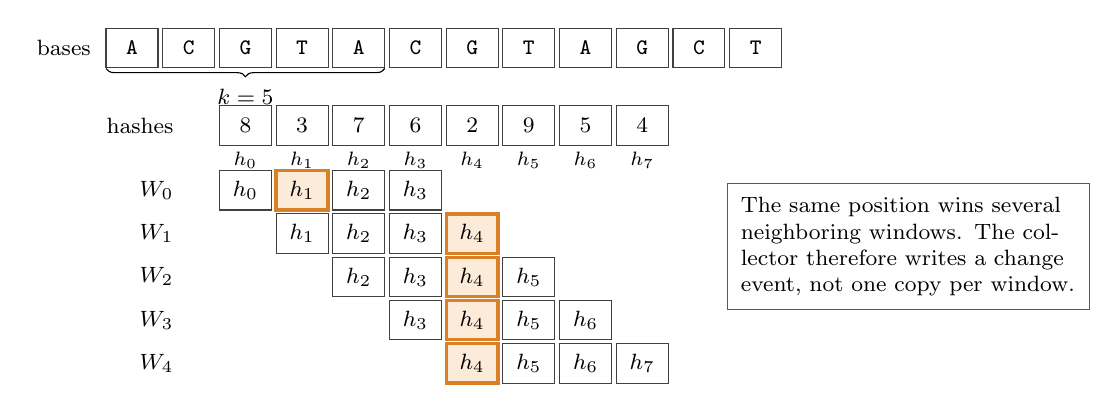
\begin{tikzpicture}[x=1cm,y=.67cm,font=\footnotesize]
  \foreach \i/\b in {0/A,1/C,2/G,3/T,4/A,5/C,6/G,7/T,8/A,9/G,10/C,11/T}
    \node[rewrite cell,font=\ttfamily\footnotesize] at (.55+\i*.72,4.95) {\b};
  \node[anchor=east] at (.15,4.95) {bases};
  \draw[decorate,decoration={brace,mirror,amplitude=3pt}]
    (.22,4.56)--(3.76,4.56)
    node[midway,below=4pt] {$k=5$};

  \foreach \i/\v in {0/8,1/3,2/7,3/6,4/2,5/9,6/5,7/4}
    \node[rewrite cell] at (1.99+\i*.72,3.48) {\v};
  \node[anchor=east] at (1.20,3.48) {hashes};
  \foreach \i in {0,...,7}
    \node[font=\scriptsize,anchor=north] at (1.99+\i*.72,3.16) {$h_{\i}$};

  \foreach \row/\start/\winner in {0/0/1,1/1/4,2/2/4,3/3/4,4/4/4} {
    \pgfmathsetmacro{\yy}{2.25-.82*\row}
    \node[anchor=east] at (1.20,\yy) {$W_{\row}$};
    \foreach \j in {0,...,3} {
      \pgfmathtruncatemacro{\idx}{\start+\j}
      \pgfmathparse{int(\idx==\winner)}
      \ifnum\pgfmathresult=1
        \node[rewrite min] at (1.99+\idx*.72,\yy) {$h_{\idx}$};
      \else
        \node[rewrite cell] at (1.99+\idx*.72,\yy) {$h_{\idx}$};
      \fi
    }
  }
  \node[rewrite note,text width=4.25cm,anchor=west] at (8.10,1.18)
    {The same position wins several neighboring windows.  The collector
     therefore writes a change event, not one copy per window.};
\end{tikzpicture}
\caption{Minimizer extraction with illustrative $k=5$, $w=4$ hashes.  Each
row is one window of four adjacent $k$-mers. Orange marks the selected
position.  The hash value 2 remains selected while the window moves, so those
windows do not require repeated output.}
\label{fig:rewrite-minimap-walkthrough}
\end{figure}

Equal hashes at different positions are not duplicate records. We wanmt to keep both to guarantee higher minimizer density.

\begin{figure}[H]
\centering
\begin{tikzpicture}[font=\footnotesize]
  \node[anchor=west,font=\bfseries] at (0,4.20)
    {(a) Two positions have the same minimum hash};
  \node[anchor=east] at (1.40,3.52) {$W_0$};
  \foreach \i/\v/\sty in {0/8/rewrite cell,1/3/rewrite min,
                            2/7/rewrite cell,3/3/rewrite min}
    \node[\sty] at (1.90+.74*\i,3.52) {\v};
  \node[anchor=west] at (5.05,3.52)
    {hash 3 occurs at two different positions};

  \node[anchor=west,font=\bfseries] at (0,2.82)
    {(b) The next candidate is larger};
  \node[anchor=east] at (1.40,1.94) {$W_1$};
  \foreach \i/\v/\sty in {0/3/rewrite cell,1/7/rewrite cell,
                            2/3/rewrite min,3/9/rewrite new}
    \node[\sty] at (1.90+.74*\i,1.94) {\v};
  \node[rewrite note,text width=5.0cm,anchor=west] at (5.05,1.74)
    {The rightmost 3 remains the saved minimum.  The earlier 3 is still a
     different identity and can require its own event.};

  \draw[rewrite flow] (3.00,1.42) |- (3.95,.52);
  \node[rewrite out,minimum width=1.55cm] at (4.80,.52) {3 at right};
  \node[rewrite out,minimum width=1.70cm] at (6.65,.52) {tied 3 at left};
\end{tikzpicture}
\caption{Why a hash value alone does not define the output.  Both orange
cells have hash 3, but they refer to different $k$-mer positions.  Minimap2
keeps the rightmost equal position as its saved minimum and has explicit
rules for writing other tied identities.}
\label{fig:rewrite-minimap-ties}
\end{figure}

Minimap2 stores the most recent $w$ candidates in a circular buffer  It also
stores the current minimum and the array slot containing it.

\begin{figure}[H]
\centering
\begin{tikzpicture}[font=\footnotesize]
  \node[anchor=west,font=\bfseries] at (0,4.55) {(a) Cheap step};
  \node at (2.65,4.12) {before};
  \foreach \i/\v/\sty in {0/8/rewrite cell,1/2/rewrite min,
                            2/7/rewrite cell,3/6/rewrite cell}
    \node[\sty] at (1.55+.72*\i,3.48) {\v};
  \draw[rewrite flow] (4.18,3.48)--(4.82,3.48);
  \node[align=center] at (4.50,2.95) {drop 8\quad add 5};
  \node at (6.25,4.12) {after};
  \foreach \i/\v/\sty in {0/2/rewrite min,1/7/rewrite cell,
                            2/6/rewrite cell,3/5/rewrite new}
    \node[\sty] at (5.18+.72*\i,3.48) {\v};
  \node[rewrite note,text width=3.75cm,anchor=west] at (8.35,3.48)
    {2 is still inside the window. Compare only $5>2$: O(1) work};

  \node[anchor=west,font=\bfseries] at (0,2.18) {(b) Expensive step};
  \node at (2.65,1.75) {before};
  \foreach \i/\v/\sty in {0/2/rewrite min,1/7/rewrite cell,
                            2/6/rewrite cell,3/5/rewrite cell}
    \node[\sty] at (1.55+.72*\i,1.10) {\v};
  \draw[rewrite flow] (4.18,1.10)--(4.82,1.10);
  \node[align=center] at (4.50,.58) {drop 2\quad add 9};
  \node at (6.25,1.75) {after};
  \foreach \i/\v in {0/7,1/6,2/5,3/9}
    \node[rewrite new] at (5.18+.72*\i,1.10) {\v};
  \node[rewrite min] at (5.18+.72*2,1.10) {5};
  \draw[draw=rewriteOrange!90!black,very thick]
    (4.80,.72) rectangle (7.72,1.48);
  \node[rewrite note,text width=3.75cm,anchor=west] at (8.35,1.10)
    {2 leaves. Read all $w=4$ live slots and choose 5: $O(w)$.};
\end{tikzpicture}
\caption{The two costs of one minimap2 window advance. Gray cells are already
in the ring, blue is the entering candidate, and orange is the saved or newly
found minimum. A normal step performs one comparison. When the saved minimum
leaves, the algorithm reads the complete window again (rescan)}
\label{fig:rewrite-minimap-rescan}
\end{figure}

Minimap2 stores kmers and apply hash function each time from scratch.

\begin{algorithm}[H]
\caption{Scalar minimap2-style rescan}
\label{alg:rewrite-minimap-rescan}
\small
\begin{enumerate}
  \item Store $k$-mer binary representation and its reverse complement and update them each step. Calculate hash for both of them and take the minimum.
  \item Write this hash into the next slot of the $w$-slot circular buffer.
  \item If new hash is less than or equal to the saved minimum, emit new minimizer.
  \item Else, if the overwritten slot held the current minimum, emit new minimizer and scan all $w$ slots from oldest to newest, and save the
        rightmost record having the smallest hash as new minimum.
  \item At the end of the sequence, write the remaining saved minimum from buffer as final minimizers.
\end{enumerate}
\end{algorithm}

\section{A1: Naive SIMD rescan}
\label{sec:rewrite-naive-simd}

Let's assume we have scalar linear iteration over data. The first though is to unroll the loop so each element of a SIMD vector corresponds to one iteration. This approach however works only if each iteration step is independent.
If we have any condition that requires knowledege of results of previous step the SIMD vector's elements will be dependent on each other and won't give us any advantage. The other approach would be to threat each element not as consecutive input items, but as separate entities handling different parts of the input. Each lane will handle separate parts of iteration, so we will avoid data dependency of vector's elements on each other and replace it with the 
dependency between current state vector and previous state vector.
In this document, I will define a SIMD lane as one numbered element of a vector register.

Each SIMD lane will load fragments of input data:

\begin{figure}[H]
\centering
\begin{tikzpicture}[
  font=\footnotesize,
  context/.style={draw,fill=gray!16,minimum height=.46cm,inner sep=0pt},
  mainspan/.style={draw=blue!70!black,fill=blue!8,
                    minimum height=.46cm,inner sep=0pt},
  cell/.style={draw,minimum width=.62cm,minimum height=.46cm,inner sep=0pt},
  inputcell/.style={draw=blue!70!black,fill=blue!8,
                    minimum width=.62cm,minimum height=.46cm,inner sep=0pt},
  mincell/.style={draw=orange!85!black,very thick,fill=orange!13,
                  minimum width=.62cm,minimum height=.46cm,inner sep=0pt},
  maskcell/.style={draw,fill=gray!10,minimum width=.62cm,
                    minimum height=.42cm,inner sep=0pt},
  outcell/.style={draw=orange!85!black,thick,fill=orange!10,
                  minimum width=1.42cm,minimum height=.48cm,inner sep=2pt},
  stage/.style={draw,minimum width=2.25cm,minimum height=.96cm,
                text width=2.00cm,align=center,inner sep=3pt},
  flow/.style={-{Latex[length=1.8mm]},thick}
]
  \node[anchor=west,font=\bfseries] at (.25,10.65)
    {(a) One SIMD lane per overlapping sequence chunk};

  \foreach \r/\start in {0/1.65,1/3.35,2/5.05,3/6.75} {
    \pgfmathsetmacro{\yy}{9.95-.54*\r}
    \node[anchor=east] at (1.43,\yy) {lane \r};
    \draw[fill=gray!16] (\start,{\yy-.23})
      rectangle ({\start+.78},{\yy+.23});
    \draw[draw=blue!70!black,fill=blue!8] ({\start+.78},{\yy-.23})
      rectangle ({\start+2.48},{\yy+.23});
  }
  \draw[fill=gray!16] (9.72,10.12) rectangle (10.18,10.48);
  \node[anchor=west] at (10.32,10.30) {warm-up context};
  \draw[draw=blue!70!black,fill=blue!8]
    (9.72,9.55) rectangle (10.18,9.91);
  \node[anchor=west] at (10.32,9.73) {later lane steps};
  \node[anchor=north west,align=left,text width=3.05cm] at (9.48,9.30)
    {Chunk starts are separated.  Each read span repeats context from the
      neighbouring region.};
    
  \node[anchor=west,font=\bfseries] at (0,7.08)
    {(b) Lane 0 loses its minimum, so the shared branch scans all lanes};
  \foreach \r/\lab in {0/lane 0,1/lane 1,2/lane 2,3/lane 3}
    \node[anchor=east] at (1.35,5.35-.48*\r) {\lab};
  \foreach \r/\c/\v in {
      0/0/7,0/1/6,0/2/5,0/3/9,
      1/0/3,1/1/7,1/2/6,1/3/5,
      2/0/8,2/1/1,2/2/4,2/3/6,
      3/0/5,3/1/6,3/2/2,3/3/8}
    \node[rewrite new] at (1.80+.70*\c,5.35-.48*\r) {\v};
  \node[rewrite min] at (1.80+.70*2,5.35) {5};
  \node[rewrite box,minimum width=2.45cm] (mask) at (6.10,4.63)
    {expiry mask\\$[1,0,0,0]$};
  \draw[rewrite flow] (4.28,4.63)--(mask.west);
  \node[rewrite note,text width=4.0cm,anchor=west] at (7.55,4.63)
    {Only lane 0 accepts a replacement. The processor still loads and
     compares all four vector slots.};
  \draw[draw=rewriteOrange!90!black,very thick]
    (1.43,3.25) rectangle (4.24,5.72);
  \node[rewrite box,fill=rewriteOrange!12,minimum width=4.0cm]
    at (5.95,2.62) {$w=4$ vector loads and comparisons};
  
\end{tikzpicture}
\caption{Why direct SIMD rescan is costly. Each lane follows a different
sequence piece. A nonzero expiry mask enters one shared loop over all $w$
vector slots. Masking protects lanes 1--3 from changing their answers, but it
does not remove their loads and comparisons.}
\label{fig:rewrite-naive-simd-rescan}
\end{figure}

Note that algorithm fundamentally stays the same, we only now divided input sequence into chunks and translated each operation (hashing, comparisons) into SIMD instructions:

\begin{algorithm}[H]
\caption{SIMD minimap2-style rescan, with the output cases stated plainly}
\label{alg:simd-minimap-rescan}
\small
\begin{enumerate}
  \item Split input sequence into chunks each corresponding to the lane of SIMD vector. Each lane handles different chunk (chunks overlap slightly to make sure we don't omit any window)
  \item Store $k$-mer binary representations and its reverse complements and update them each step for each lane. Calculate hashes for both of them and take the minimum for each lane.
  \item Write all hashes for each laneinto the next slot of the $w$-slot circular buffer (this buffer now stores SIMD vectors instead of single hashes).
  \item If the new hash vector is less than equal to the minimum vector element-wise, extract corresponding elements and emit new minimizers.
  \item Else (new hash vector is greater then minimum vector on each position), if the overwritten slot held the current minimum for any lane, emit new minimizers and scan all $w$ slots from oldest to newest, and save the
        new minimums vector.
  \item At the end of the sequence, emit all remaining minimums as final minimizers.
\end{enumerate}
\end{algorithm}

As you can see this algorithm works well only if new hash values are greater than current minimum on each position. If not, we still have branching. This is problematic as vectorized algorithms works well if the branching is minimal and CPU pipeline isn't penalized for wrong branch prediction.
Even if we assume the predictor is perfect, we still do expensive rescan for each lane if at least one needs to be updated. Assume one lane needs a rescan with probability $1/w$, then a group of $L$
independent lanes enters the shared slow path with probability
\[
  1-\left(1-\frac1w\right)^L.
\]
For $w=10$ and $L=4$, this is about $34.4\%$. This means that we will need to duplicate work much more often than in scalar case.

\section{A2: Two-stack algorithm}
\label{sec:rewrite-sea-simd-minimizers}

In different approach we can preserve prefix and suffix minima to calculate the window minima wrom both of them. SIMD-minimizers paper introduces this approach as well as usage of rolling hashes (nthash) instead of calculating hash each time from scratch. \cite{groot_koerkamp_simd_minimizers_2025}

\subsection{One window minimum from two saved values}

Split the hash stream into blocks of $w$ values.  Within each block, let
$P_i$ be the smallest value from the block start through position $i$, and let
$Q_i$ be the smallest value from position $i$ through the block end.  A window
starting at $j$ and ending at $e=j+w-1$ crosses one block boundary and has
minimum
\[
  \min(Q_j,P_e).
\]
The suffix values are recalculated in a fixed $w$-step loop each $w$ steps. This means that we still have "rescan" part, but it becames unconditional.


\begin{figure}[H]
\centering
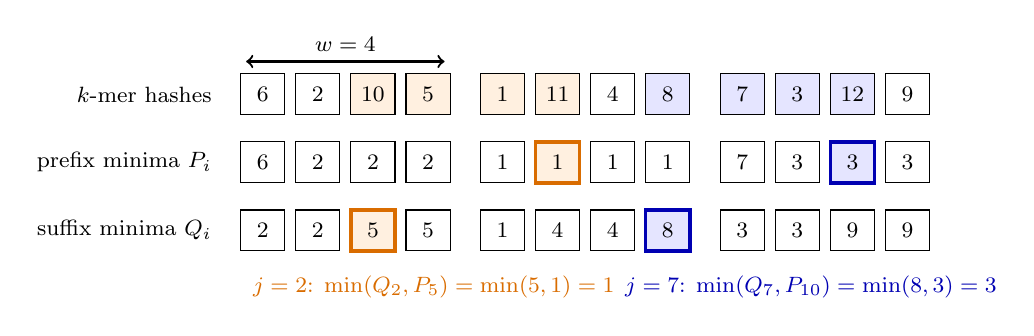
\begin{tikzpicture}[
  x=.70cm,
  y=.72cm,
  font=\footnotesize,
  cell/.style={draw,minimum width=.56cm,minimum height=.52cm,inner sep=0pt},
  first/.style={draw=orange!85!black,very thick,fill=orange!12,
                minimum width=.56cm,minimum height=.52cm,inner sep=0pt},
  second/.style={draw=blue!70!black,very thick,fill=blue!10,
                  minimum width=.56cm,minimum height=.52cm,inner sep=0pt}
]
  \node[anchor=east] at (4.25,3.25) {$k$-mer hashes};
  \foreach \i/\x/\v in {0/5.00/6,1/6.00/2,2/7.00/10,3/8.00/5,
                            4/9.35/1,5/10.35/11,6/11.35/4,7/12.35/8,
                            8/13.70/7,9/14.70/3,10/15.70/12,11/16.70/9}
    \node[cell] (a\i) at (\x,3.25) {\v};
  \foreach \i/\x/\v in {2/7.00/10,3/8.00/5,4/9.35/1,5/10.35/11}
    \node[cell,fill=orange!12] at (\x,3.25) {\v};
  \foreach \i/\x/\v in {7/12.35/8,8/13.70/7,9/14.70/3,10/15.70/12}
    \node[cell,fill=blue!10] at (\x,3.25) {\v};
  \draw[<->,thick] (4.70,3.83) -- (8.30,3.83)
    node[midway,above] {$w=4$};

  \node[anchor=east] at (4.25,2.05) {prefix minima $P_i$};
  \foreach \i/\x/\v in {0/5.00/6,1/6.00/2,2/7.00/2,3/8.00/2,
                            4/9.35/1,5/10.35/1,6/11.35/1,7/12.35/1,
                            8/13.70/7,9/14.70/3,10/15.70/3,11/16.70/3}
    \node[cell] (p\i) at (\x,2.05) {\v};
  \node[first] at (10.35,2.05) {1};
  \node[second] at (15.70,2.05) {3};

  \node[anchor=east] at (4.25,.85) {suffix minima $Q_i$};
  \foreach \i/\x/\v in {0/5.00/2,1/6.00/2,2/7.00/5,3/8.00/5,
                            4/9.35/1,5/10.35/4,6/11.35/4,7/12.35/8,
                            8/13.70/3,9/14.70/3,10/15.70/9,11/16.70/9}
    \node[cell] (q\i) at (\x,.85) {\v};
  \node[first] at (7.00,.85) {5};
  \node[second] at (12.35,.85) {8};

  \node[anchor=west,orange!85!black] at (4.65,-.15)
    {$j=2$: $\min(Q_2,P_5)=\min(5,1)=1$};
  \node[anchor=west,blue!70!black] at (11.40,-.15)
    {$j=7$: $\min(Q_7,P_{10})=\min(8,3)=3$};
\end{tikzpicture}
\caption{Sliding minima from blockwise prefixes and suffixes. The two shaded crossing windows each use
one suffix value from the starting block and one prefix value from the ending
block.}
\label{fig:two-stack-minimum}
\end{figure}

\info{Fixed-width SIMD vectors}{The SIMD-Minimizers use fixed-vector size architecture, where the SIMD vector is set to be uint32 times 8. The split per lane is the same as discussed previously. On Neon architecture only 128-bit-wide register is available, so the 256 fixed vector generates separate store intructions.}

\begin{figure}[H]
\centering
\begin{tikzpicture}[
  x=.64cm,
  y=.68cm,
  font=\footnotesize,
  >=Latex,
  owned/.style={draw=blue!70!black,fill=blue!10,minimum height=.58cm},
  halo/.style={draw=orange!80!black,fill=orange!12,minimum height=.58cm},
  stage/.style={draw,rounded corners,fill=gray!8,align=center,
                minimum width=2.25cm,minimum height=1.05cm,inner sep=3pt}
]
  \node[anchor=east] at (1.30,6.05) {sequence $S$};
  \draw[thick] (1.55,5.72) rectangle (19.65,6.38);
  \foreach \x in {5.55,9.55,13.55,17.55}
    \draw[gray!70] (\x,5.72) -- (\x,6.38);
  \foreach \x/\v in {3.55/$C_0$,7.55/$C_1$,11.55/$C_2$,15.55/$C_3$}
    \node at (\x,6.05) {\v};
  \node at (18.60,6.05) {$\cdots$};

  \draw[owned] (1.55,4.55) rectangle (5.55,5.13);
  \draw[halo] (5.55,4.55) rectangle (7.55,5.13);
  \node at (3.55,4.84) {$C_0$ owned};
  \node at (6.55,4.84) {context};
  \draw[owned] (5.55,3.65) rectangle (9.55,4.23);
  \draw[halo] (9.55,3.65) rectangle (11.55,4.23);
  \node at (7.55,3.94) {$C_1$ owned};
  \node at (10.55,3.94) {context};
  \node[anchor=west] at (12.05,4.38)
    {$g=k+w-2$ bases of context};
  \node[anchor=west,gray!75] at (12.05,3.82)
    {remaining chunks follow the same rule};
  \draw[->] (3.55,5.70) -- (3.55,5.16);
  \draw[->] (7.55,5.70) -- (7.55,4.27);

  \node[stage] (lanes) at (2.15,1.55)
    {lane matrix\\$C_0[t]\quad C_1[t]$\\$C_2[t]\quad C_3[t]$};
  \node[stage] (hash) at (6.25,1.55)
    {rolling hashes\\$h_{0,t}\quad h_{1,t}$\\$h_{2,t}\quad h_{3,t}$};
  \node[stage] (minimum) at (10.35,1.55)
    {window argmin\\$p_{0,t}\quad p_{1,t}$\\$p_{2,t}\quad p_{3,t}$};
  \node[stage] (absolute) at (14.45,1.55)
    {absolute positions\\$p_{c,t}+o_c$};
  \node[stage] (collect) at (19.05,1.55)
    {collected output\\$p_0,p_1,p_2,\ldots$\\deduplicate identity};
  \draw[->,thick] (lanes) -- (hash);
  \draw[->,thick] (hash) -- (minimum);
  \draw[->,thick] (minimum) -- (absolute);
  \draw[->,thick] (absolute) -- (collect);
  \draw[->,thick] (7.55,3.55) to[out=-90,in=90] (lanes.north);
\end{tikzpicture}
\caption{Vectorized minimizer extraction: Each chunk owns
a disjoint range and reads enough context to complete its windows.}
\label{fig:vector-minimizer-pipeline}
\end{figure}


Note that in this setup we can store full minimum vectors and later use matrix transposition to deduplicate them (in case that minimum stays the same over window):
At first, one SIMD vector contains the selected positions for several
far-apart streams at the same step.  After several steps, the SIMD-Minimizers paper algorithm
rearranges that output matrix so one row contains consecutive windows from
one stream.  Consecutive windows often select the same position.  Once those
positions are adjacent in a row, the paper compares neighbors and keeps only
positions that changed.  Finally, when the ordered stream results are joined,
it removes the repeated boundary position caused by the overlapping input
pieces.


\begin{figure}[H]
\centering
\begin{tikzpicture}[
  x=.62cm,
  y=.62cm,
  font=\footnotesize,
  >=Latex,
  cell/.style={draw,minimum width=.52cm,minimum height=.52cm,inner sep=0pt},
  trace/.style={draw=orange!85!black,very thick,fill=orange!12,
                minimum width=.52cm,minimum height=.52cm,inner sep=0pt},
  carry/.style={draw=gray!70,fill=gray!10,text=gray!80,
                minimum width=.52cm,minimum height=.52cm,inner sep=0pt}
]
  \node[font=\small\bfseries] at (2.50,4.15) {events by vector step};
  \foreach \r/\c/\v in {0/0/1,0/1/12,0/2/23,0/3/30,
                            1/0/1,1/1/13,1/2/23,1/3/35,
                            2/0/2,2/1/13,2/2/23,2/3/35,
                            3/0/4,3/1/13,3/2/23,3/3/36}
    \node[cell] at (1+\c,3-\r) {\v};
  \foreach \r/\v in {0/1,1/1,2/2,3/4}
    \node[trace] at (1,3-\r) {\v};

  \node[font=\small\bfseries] at (9.50,4.15) {one sorted row per chunk};
  \foreach \r/\c/\v in {0/0/1,0/1/1,0/2/2,0/3/4,
                            1/0/12,1/1/13,1/2/13,1/3/13,
                            2/0/23,2/1/23,2/2/23,2/3/23,
                            3/0/30,3/1/35,3/2/35,3/3/36}
    \node[cell] at (8.0+\c,3-\r) {\v};
  \foreach \c/\v in {0/1,1/1,2/2,3/4}
    \node[trace] at (8.0+\c,3) {\v};

  \draw[->,very thick] (5.00,1.5) -- (7.20,1.5)
    node[midway,above] {transpose};
  \draw[->,very thick] (11.80,1.5) -- (14.85,1.5)
    node[midway,above,align=center] {deduplicate\\and append};

  \node[font=\small\bfseries] at (17.5,4.15) {ragged chunk outputs};
  \node at (15.6,3.65) {$\operatorname{last}[c]$};
  \foreach \r/\v in {0/0,1/11,2/23,3/30}
    \node[carry] at (15.6,3-\r) {\v};
  \foreach \x/\v in {16.9/1,17.9/2,18.9/4}
    \node[trace] at (\x,3) {\v};
  \foreach \x/\v in {16.9/12,17.9/13}
    \node[cell] at (\x,2) {\v};
  \node[anchor=west,gray!75] at (16.65,1) {no new position};
  \foreach \x/\v in {16.9/35,17.9/36}
    \node[cell] at (\x,0) {\v};
  \foreach \r in {0,...,3}
    \draw[->,gray!70] (15.95,3-\r) -- (16.50,3-\r);
\end{tikzpicture}
\caption{Transposition and boundary deduplication for four logical chunks.
The input rows are vector steps and the columns are chunks. Transposition
makes each chunk a sorted row. Each row has its own previous-position carry,
shown in gray. Only new positions are appended, so padding cells are not part
of the output.}
\label{fig:transpose-dedup}
\end{figure}

\section{A3: Chronological SIMD}
\label{sec:rewrite-v8}

Looking at A1 we observed that the main problem was that far-apart sequence chunks can have different characterisistics which cause us to do lots of additional work. Instead of splitting sequence that way, we can work on just one part of neighbouring positions.

We will try to calculate minimums for all local windows i.e calculate result for $X[p, p+1, ..., p+k+w-1]$ (this is window of size $w$ for kmers of size $k$).
Physically we only have $L$ SIMD lanes so we will call that a group and advance only by $L$ positions at the time (i.e from $X[p, p+1, ..., p+k+w-1]$ to $X[p+L, p+L+1, ..., p+k+w-1+L]$).

Potentially we can have more than one group per call. It offers some advantages discussed later. If the group number is higher, then we just execute their operations serially and perform result emission only after all groups execute.

The idea for one group is as follows:
\begin{enumerate}
  \item We load $L$ new sequence positions into $L$ SIMD lanes each one is shifted by $1$ using load instructions
  \item For each lane we compute minimum along with strand direction and information which position it is. We call that new candidates: $x_0,\ldots,x_{L-1}$
  \item We iterate through all candidates i.e $D\gets T\mathbin\Vert(x_0,\ldots,x_{L-1})$ where $T$ are previous $w-1$ candidates and calculate new minimums. This gives us $M$ which are $L$ minimums for entire parts of sequence:
  \[
    \begin{aligned}
      \{&\operatorname{Seed}(X[p,p+1,\ldots,p+k+w-1]),\\
        &\operatorname{Seed}(X[p+1,p+2,\ldots,p+k+w]),\ldots,\\
        &\operatorname{Seed}(X[p+L,p+L+1,\ldots,p+k+w+L])\}.
    \end{aligned}
  \]
  Now this along last previous result $c^{*}$ forms $P$: $\mathbf P\gets(c^\star,M_0,\ldots,M_{L-2})$
  \item For each lane $\ell$ we compare $P_{\ell}$ with $x_{\ell}$. If $h(x_{\ell}) \leq P_{\ell}$ then $P_{\ell}$ is a new minimizer and we emit it. Otherwise if $\text{pos}(P_{\ell}) = \text{pos}(x_{\ell})$ then we see $P_{\ell}$ expired so we emit it. 
  \item If the expiry happens then we go through all $w$ windows and check if their minimum has the same value but different position. This only requires checking $m_0, m_1, ..., m_{w-1}$. If yes then we do slow path: extract the ties in order (hence the name of the algorithm: chronological)
\end{enumerate}

\begin{figure}[H]
  \centering
  \begin{tikzpicture}[
    x=1cm,
    y=.55cm,
    font=\footnotesize,
    >=Latex,
    cell/.style={draw=black!68,minimum width=.43cm,
      minimum height=.34cm,inner sep=0pt},
    retained/.style={cell,fill=rewriteGray!18},
    entering/.style={cell,draw=rewriteBlue!90!black,
      fill=rewriteBlue!14},
    padding/.style={cell,draw=rewriteGray!75,dashed,
      fill=rewriteGray!5,text=rewriteGray!85!black},
    winner/.style={cell,draw=rewriteOrange!95!black,very thick,
      fill=rewriteOrange!22},
    earlier/.style={cell,draw=rewriteOrange!95!black,densely dashed,
      fill=rewriteOrange!7},
    group/.style={draw=rewriteBlue!90!black,very thick,
      fill=rewriteBlue!10,rounded corners,minimum width=1.05cm,
      minimum height=.52cm,inner sep=2pt},
    result/.style={draw=rewriteOrange!95!black,very thick,
      fill=rewriteOrange!13,rounded corners,minimum width=1.48cm,
      minimum height=.30cm,inner xsep=2pt,inner ysep=0pt},
    state/.style={draw=rewriteGreen!75!black,fill=rewriteGreen!11,
      rounded corners,minimum height=.50cm,inner sep=3pt},
    flow/.style={-{Latex[length=1.8mm]},thick},
    softflow/.style={-{Latex[length=1.6mm]},thick,
      draw=rewriteGray!90!black}
  ]
  
  % --------------------------------------------------------------------------
  % (a) Working sets and the number of groups in one full call.
  % --------------------------------------------------------------------------
  \node[anchor=west,font=\bfseries] at (0,31.10)
    {(a) Working sets and group count};
  
  \node[anchor=east] at (2.35,29.95) {generic bases};
  \node[retained,minimum width=3.55cm] (gbold) at (4.35,29.95)
    {$k-1$ retained};
  \node[entering,minimum width=2.25cm] (gbnew) at (7.55,29.95)
    {$L$ new};
  \draw[flow] (gbnew.east)--(9.30,29.95);
  \node[anchor=west] at (9.45,29.95)
    {$k$ construction steps $\longrightarrow L$ hashes};
  \node[anchor=west,text=rewriteGray!90!black] at (2.58,29.18)
    {$(k-1)+L$ live base ranks};
  
  \node[anchor=east] at (2.35,28.10) {generic: $1$ group};
  \node[retained,minimum width=3.55cm] (gcold) at (4.35,28.10)
    {$w-1$ retained};
  \node[entering,minimum width=2.25cm] (gcnew) at (7.55,28.10)
    {$L$ new};
  \draw[flow] (gcnew.east)--(9.32,28.10);
  \node[group] (ggroup) at (10.15,28.10) {$G_0$};
  \draw[flow] (ggroup.east)--(11.55,28.10);
  \node[result,minimum width=2.15cm] at (12.85,28.10) {$L$ minima};
  \node[anchor=west,text=rewriteGray!90!black] at (2.58,27.33)
    {$(w-1)+L$ candidate records};
  
  \node[anchor=east] at (2.35,26.25) {fast base scratch};
  \node[retained,minimum width=3.55cm] (fbold) at (4.35,26.25)
    {$14$ retained};
  \node[entering,minimum width=2.25cm] (fbnew) at (7.55,26.25)
    {$8$ new};
  \node[padding,minimum width=.72cm] at (9.25,26.25) {$2$};
  \node[anchor=west] at (9.85,26.25)
    {$24$ bytes: $22$ live $+2$ safety};
  
  \node[anchor=east] at (2.35,24.80) {fast: $2$ groups};
  \node[entering,minimum width=1.55cm] (firstfour) at (3.40,24.80)
    {first $4$};
  \draw[flow] (firstfour.east)--(4.80,24.80);
  \node[group] (gzero) at (5.45,24.80) {$G_0$};
  \draw[flow] (gzero.east)--(6.55,24.80);
  \node[state,minimum width=1.35cm] (update) at (7.45,24.80) {update};
  \draw[flow] (update.east)--(8.45,24.80);
  \node[entering,minimum width=1.55cm] (nextfour) at (9.40,24.80)
    {next $4$};
  \draw[flow] (nextfour.east)--(10.80,24.80);
  \node[group] (gone) at (11.45,24.80) {$G_1$};
  \draw[flow] (gone.east)--(12.55,24.80);
  \node[result,minimum width=1.80cm] at (13.65,24.80) {$4+4$ minima};
  % --------------------------------------------------------------------------
  % (b) Definition of one group.
  % --------------------------------------------------------------------------
  \node[anchor=west,font=\bfseries] at (0,22.55)
    {(b) One group reduces $L$ adjacent windows};
  
  \node[anchor=east] at (2.35,21.35) {$T=$};
  \node[retained,minimum width=3.55cm] (dold) at (4.35,21.35)
    {$w-1$ retained};
  \node[entering,minimum width=2.25cm] (dnew) at (7.55,21.35)
    {$L$ new};
  \node[anchor=west] at (9.15,21.35)
    {length $(w-1)+L$};
  
  \draw[softflow] (5.95,20.90)--(5.95,20.15);
  \node[cell,minimum width=1.12cm] at (3.30,19.65) {$V_0$};
  \node[cell,minimum width=1.12cm] at (4.75,19.65) {$V_1$};
  \node at (6.05,19.65) {$\cdots$};
  \node[cell,minimum width=1.35cm] at (7.55,19.65) {$V_{w-1}$};
  \draw[flow] (8.35,19.65)--(9.55,19.65);
  \node[result,minimum width=3.15cm] at (11.40,19.65)
    {$M=(m_t,\ldots,m_{t+L-1})$};
  
  \node[anchor=west] at (2.55,18.70)
    {$V_r=(D_s,\ldots,D_{s+L-1}),\quad s=0,\ldots,w-1$};
  \node[anchor=west,text=rewriteOrange!95!black] at (9.55,18.70)
    {$M=\min_{\leq}(V_0,\ldots,V_{w-1})$};
  
  \node[state,minimum width=1.65cm] at (3.55,17.55) {advance by $L$};
  \node[anchor=west] at (4.65,17.55)
    {tail $\gets D_L,\ldots,D_{L+w-2}$};
  \node[anchor=west] at (10.25,17.55)
    {current $\gets m_{t+L-1}$};
  
  % --------------------------------------------------------------------------
  % (c) First concrete four-window group.
  % --------------------------------------------------------------------------
  \node[anchor=west,font=\bfseries] at (0,16.20)
    {(c) Group $G_0$: first four new hashes};
  
  \node[anchor=east] at (1.78,15.15) {input};
  \foreach \i/\v/\sty in {
    0/8/retained,1/6/retained,2/5/retained,3/9/retained,
    4/4/retained,5/7/retained,6/4/retained,7/8/retained,
    8/3/retained,9/6/entering,10/3/entering,11/5/entering,
    12/2/entering}
    \node[\sty] at (2.10+.55*\i,15.15) {\v};
  \node[anchor=west,text=rewriteGray!90!black] at (9.15,15.15)
    {$D_0,\ldots,D_8$};
  \node[anchor=west,text=rewriteBlue!90!black] at (11.35,15.15)
    {$D_9,\ldots,D_{12}$};
  
  \node[anchor=east] at (2.72,14.28) {step $r$};
  \foreach \j in {0,...,9}
    \node[font=\scriptsize] at (3.10+.55*\j,14.28) {\j};
  \node[font=\scriptsize] at (9.55,14.28) {window minimum};
  
  \node[anchor=east] at (2.72,13.55) {$W_0$};
  \foreach \j/\v/\sty in {
    0/8/cell,1/6/cell,2/5/cell,3/9/cell,4/4/cell,
    5/7/cell,6/4/cell,7/8/cell,8/3/winner,9/6/cell}
    \node[\sty] at (3.10+.55*\j,13.55) {\v};
  \node[result] at (9.55,13.55) {$3@D_8$};
  
  \node[anchor=east] at (2.72,12.87) {$W_1$};
  \foreach \j/\v/\sty in {
    0/6/cell,1/5/cell,2/9/cell,3/4/cell,4/7/cell,
    5/4/cell,6/8/cell,7/3/earlier,8/6/cell,9/3/winner}
    \node[\sty] at (3.10+.55*\j,12.87) {\v};
  \node[result] at (9.55,12.87) {$3@D_{10}$};
  
  \node[anchor=east] at (2.72,12.19) {$W_2$};
  \foreach \j/\v/\sty in {
    0/5/cell,1/9/cell,2/4/cell,3/7/cell,4/4/cell,
    5/8/cell,6/3/earlier,7/6/cell,8/3/winner,9/5/cell}
    \node[\sty] at (3.10+.55*\j,12.19) {\v};
  \node[result] at (9.55,12.19) {$3@D_{10}$};
  
  \node[anchor=east] at (2.72,11.51) {$W_3$};
  \foreach \j/\v/\sty in {
    0/9/cell,1/4/cell,2/7/cell,3/4/cell,4/8/cell,
    5/3/cell,6/6/cell,7/3/cell,8/5/cell,9/2/winner}
    \node[\sty] at (3.10+.55*\j,11.51) {\v};
  \node[result] at (9.55,11.51) {$2@D_{12}$};
  
  \draw[decorate,decoration={brace,mirror,amplitude=3pt}]
    (2.80,11.08)--(8.35,11.08)
    node[midway,below=3pt,xshift=.65cm] {$w$ SIMD reduction steps};
  \node[anchor=west,text=rewriteOrange!95!black] at (10.75,12.72)
    {solid: rightmost winner};
  \node[anchor=west,text=rewriteOrange!95!black] at (10.75,12.02)
    {dashed: earlier tie};
  
  \node[state,minimum width=1.65cm] at (3.55,9.83) {advance by $L$};
  \node[anchor=west] at (4.65,9.83)
    {tail $\gets(D_4,\ldots,D_{12})$};
  \node[anchor=west] at (10.25,9.83)
    {current $\gets2@D_{12}$};
  
  % --------------------------------------------------------------------------
  % (d) Second concrete four-window group.
  % --------------------------------------------------------------------------
  \node[anchor=west,font=\bfseries] at (0,8.55)
    {(d) Group $G_1$: remaining four hashes, after the state update};
  
  \node[anchor=east] at (1.78,7.52) {input};
  \foreach \i/\v/\sty in {
    0/4/retained,1/7/retained,2/4/retained,3/8/retained,
    4/3/retained,5/6/retained,6/3/retained,7/5/retained,
    8/2/retained,9/7/entering,10/1/entering,11/9/entering,
    12/1/entering}
    \node[\sty] at (2.10+.55*\i,7.52) {\v};
  \node[anchor=west,text=rewriteGray!90!black] at (9.15,7.52)
    {$D_4,\ldots,D_{12}$};
  \node[anchor=west,text=rewriteBlue!90!black] at (11.35,7.52)
    {$D_{13},\ldots,D_{16}$};
  
  \node[anchor=east] at (2.72,6.65) {step $r$};
  \foreach \j in {0,...,9}
    \node[font=\scriptsize] at (3.10+.55*\j,6.65) {\j};
  \node[font=\scriptsize] at (9.55,6.65) {window minimum};
  
  \node[anchor=east] at (2.72,5.92) {$W_4$};
  \foreach \j/\v/\sty in {
    0/4/cell,1/7/cell,2/4/cell,3/8/cell,4/3/cell,
    5/6/cell,6/3/cell,7/5/cell,8/2/winner,9/7/cell}
    \node[\sty] at (3.10+.55*\j,5.92) {\v};
  \node[result] at (9.55,5.92) {$2@D_{12}$};
  
  \node[anchor=east] at (2.72,5.24) {$W_5$};
  \foreach \j/\v/\sty in {
    0/7/cell,1/4/cell,2/8/cell,3/3/cell,4/6/cell,
    5/3/cell,6/5/cell,7/2/cell,8/7/cell,9/1/winner}
    \node[\sty] at (3.10+.55*\j,5.24) {\v};
  \node[result] at (9.55,5.24) {$1@D_{14}$};
  
  \node[anchor=east] at (2.72,4.56) {$W_6$};
  \foreach \j/\v/\sty in {
    0/4/cell,1/8/cell,2/3/cell,3/6/cell,4/3/cell,
    5/5/cell,6/2/cell,7/7/cell,8/1/winner,9/9/cell}
    \node[\sty] at (3.10+.55*\j,4.56) {\v};
  \node[result] at (9.55,4.56) {$1@D_{14}$};
  
  \node[anchor=east] at (2.72,3.88) {$W_7$};
  \foreach \j/\v/\sty in {
    0/8/cell,1/3/cell,2/6/cell,3/3/cell,4/5/cell,
    5/2/cell,6/7/cell,7/1/earlier,8/9/cell,9/1/winner}
    \node[\sty] at (3.10+.55*\j,3.88) {\v};
  \node[result] at (9.55,3.88) {$1@D_{16}$};
  
  \draw[decorate,decoration={brace,mirror,amplitude=3pt}]
    (2.80,3.45)--(8.35,3.45)
    node[midway,below=3pt,xshift=.65cm] {$w$ SIMD reduction steps};
  
  \node[state,minimum width=1.65cm] at (3.55,2.18) {advance by $L$};
  \node[anchor=west] at (4.65,2.18)
    {tail $\gets(D_8,\ldots,D_{16})$};
  \node[anchor=west] at (10.25,2.18)
    {current $\gets1@D_{16}$};
  
  \node[align=center,text width=4.8cm,text=rewriteBlue!90!black,
        font=\small] at (2.80,.72)
    {$8$ window minima in two groups $G_0$ and $G_1$};
  \node[align=center,text width=2.8cm,text=rewriteOrange!95!black,
        font=\small] at (7.20,.72)
    {$2w$ reductions};
  \node[align=center,text width=4.0cm,text=rewriteGreen!75!black,
        font=\small] at (11.80,.72)
    {hash ties are resolved separately};
  
  \end{tikzpicture}
  \caption{Working sets and execution of the chronological adjacent-window
  kernel.  One group combines previous $w-1$ candidates with $L$ new
  candidates, then loads $w$ shifted vectors, and reduces them componentwise to the
  rightmost minima of $L$ adjacent windows. Orange cells represent selected minimums (candidates for potential minimizer emit).
  A solid orange cell is the rightmost equal minimum selected by the source's $\leq$ comparison and a dashed cell is an earlier equal
  minimum.}
  \label{fig:rewrite-chronological-groups}
  \end{figure}
  
The figure \ref{fig:rewrite-chronological-groups} illustrates calculation of window minima for $L=4$ lanes: $x_0, x_1, ... x_{L-1}$. The entire algorithm looks as follows:

  \begin{algorithm}[H]
  \caption{One iteration: build $L$ $k$-mers and rescan $L$ adjacent windows}
  \label{alg:rewrite-generic-chronological}
  \footnotesize
  \begin{algorithmic}[1]
  \State \textbf{Carry:} $C$ = last $k-1$ bases,
         $T$ = last $w-1$ candidates,
         $c^\star$ = preceding window minimum
  \While{the next $L$ candidate bases are available}
    \State $U\gets$ next $L$ bases
    \State $Y\gets C\mathbin\Vert U$
    \State $\mathbf F,\mathbf R\gets\mathbf0$
    \AlgCommentLine{Build forward/reverse kmers symbol by symbol.}
    \For{$t=0,\ldots,k-1$}
      \State $\mathbf z\gets\operatorname{load}_L(Y[t\,..\,t+L))$
      \State $\mathbf F\gets F\mathbin\Vert z$
      \State $\mathbf R\gets\overline{z}\mathbin\Vert R$
    \EndFor
    \AlgCommentLine{Calculate hashes from kmers.}
    \ForAll{lanes $\ell$}
      \State $a_\ell\gets H(\min(F_\ell,R_\ell))$
      \If{$F_\ell=R_\ell$ or $a_\ell=h_{\max}$}
        \State $x_\ell\gets\infty$
      \Else
        \State $x_\ell\gets\operatorname{pack}
          (a_\ell,\operatorname{position}_\ell,[R_\ell<F_\ell])$
      \EndIf
    \EndFor
    \State $D\gets T\mathbin\Vert(x_0,\ldots,x_{L-1})$
    \State $\mathbf M\gets\infty$
    \AlgCommentLine{Calculate $M$, which holds the rightmost minima of all $w$ windows.}
    \For{$s=0,\ldots,w-1$}
      \State $\mathbf V\gets D[s\,..\,s+L)$
      \State $\mathbf M\gets
        \operatorname{select}(h(\mathbf V)\leq h(\mathbf M),
                              \mathbf V,\mathbf M)$
    \EndFor
    \AlgCommentLine{One step = three field loads + one compare + three selects.}
    \State Hence $M_\ell$ is the rightmost minimum of the complete window
           ending at $x_\ell$
    \State $\mathbf P\gets(c^\star,M_0,\ldots,M_{L-2})$
    \ForAll{lanes $\ell$}
      \State $e\gets\emptyset$
      \If{$x_\ell=P_\ell$}
        \State $e\gets\operatorname{event}^{\mathrm{NEW}}(P_\ell)$
      \EndIf
      \If{$\operatorname{pos}(P_\ell)=\operatorname{pos}(x_\ell)$}
        \State $e\gets\operatorname{event}^{\mathrm{EXPIRED}}(P_\ell)$
              \Comment{expiration}
      \EndIf
      \If{$e$ is \textsc{Expired}}
        \State Check all $w$ windows for an equal hash on a different position
        \State $e\gets\operatorname{event}^{\mathrm{TIE}}(P_\ell)$
      \EndIf
      \If{$e$ is \textsc{Tie}}
        \State Reread the $w$ records only to construct ordered output
              \Comment{slow path}
      \EndIf
    \EndFor
    \State $C\gets Y[L\,..\,L+k-1)$
    \State $T\gets D[L\,..\,L+w-1)$
    \State $c^\star\gets M_{L-1}$
  \EndWhile
  \If{$0<q<L$ bases remain}
    \State Run the same body once with $q$ active lanes and sentinels elsewhere
    \State Both loops still execute $k$ and $w$ steps
    \State $C\gets Y[q\,..\,q+k-1)$,
           $T\gets D[q\,..\,q+w-1)$,
           $c^\star\gets M_{q-1}$
  \EndIf
  \end{algorithmic}
  \end{algorithm}
  
\section{Bioseq prototype}

We established different approaches to calculate minimizers in previous sections.Now we want to discuss practical considerations when it comes to implementing those algorithms.
The work started by exploring minimap2 source code and understanding its behaviour. The first step was to port minimap2 code into modern C++. This was required to have a stable code where we could test and benchmark different algorithms.
I encountered several key problems that lagged implementation by considerable number of months:
\begin{enumerate}
  \item Minimap2 code uses direct C arrays access for lots of different data structures. Minimizers are encoded as uint128 type represented by a struct with two uint64 fields with abstract filed names. Circular buffers are represented by single raw pointer and require macros for any operations. The encoding and semantics of fields can sometimes change even though underlying uint128 representation stays the same (it's the same field name). This complicates any manual static analysis of the code I conducted.
  \item Minimap2 uses raw instrinsics for SIMD operations which makes translation to generic SIMD very tedious.
  \item Some parts of minimap2 hash logic are undocumented either in official paper or in-code.
\end{enumerate}

The porting involved several iterations over the minimap2 source to understand how index is split, how parallelization works and how exactly minimizers are represented.
After achieving runnable pipeline (with seeding, chaining, alignment and estimator) I started to work specifically on the minimizer extraction part as it's first in the pipeline.


\begin{table}[H]
  \centering
  \footnotesize
  \begin{tabularx}{\linewidth}{@{}p{.13\linewidth}X@{}}
  \toprule
  Label & \shortstack[l]{Main change\\What it means for the minimizer algorithm} \\
  \midrule
  V1--V6 & naive SIMD rescan approach equivalent to A1 \\
  V7--V8 & hybrid algorithm A1 where we use two-stack for minimum calculation \\
  V8.5 & defer minimap2 hashing to later stages \\
  V9-V10 & hand-written input and matrix loop \\
  V11 & two independent Highway lane groups \\
  V12 & force the per-base body inline \\
  V13 & fixes of estimator \\
  \bottomrule
  \end{tabularx}
  \caption{History of the first prototypes}
  \label{tab:rewrite-version-history}
  \end{table}


\section{Seeding prototype V1--V6: Naive SIMD rescan}
\label{sec:v6-rescan}

The first approach (apart from direct minimap2 scalar rescan already existing in the ported code) was implementation of A1 SIMD rescan.

As correctly predicted our benchmark (Table~\ref{tab:v6-phase}) showed that the scalar
\texttt{mm\_sketch} took 12.5\,ms on a 903\,kbp pair, while the
``vectorised'' \texttt{mm\_sketch\_simd} took 24\,ms -- a 2$\times$
slowdown. This was caused by the fact that any minimum going outside the window causes rescan of all lanes.

\begin{table}[H]
  \centering
  \begin{tabular}{lrrr}
    \toprule
    Phase & scalar (ms) & V6 SIMD (ms) & V6 over scalar \\
    \midrule
    \texttt{mm\_sketch}      & 12.50 & 14.94 & $+19\,\%$ \\
    \texttt{mm\_sketch\_simd} & 0    & 23.88 & --- \\
    \texttt{target\_index\_build} & 16.0 & 14.3 & $-11\,\%$ \\
    \texttt{collect\_seed\_hits} & 6.5  & 11.0 & $+69\,\%$ \\
    \texttt{mg\_lchain\_dp}   & 16.0 & 0.0  & --- (replaced) \\
    \texttt{mg\_lchain\_simd} & 0.0  & 8.9  & --- \\
    \texttt{mm\_est\_err}     & 0.7  & 7.2  & $+929\,\%$ \\
    \texttt{mm\_align\_skel.}  & 87.5 & 86.4 & $-1\,\%$ \\
    \midrule
    Pipeline total per pair & 158.4 & 170.7 & $+8\,\%$ \\
    \bottomrule
  \end{tabular}
  \caption{Phase breakdown at 903\,kbp, V3 baseline -- pre-SIMD-Minimizers
    work. The naive SIMD path (V6) is $+8\,\%$ \emph{slower} than
    scalar despite four lanes of parallelism. The slowdown is split
    between three regressions: (a) the SIMD minimizer's
    \texttt{mm\_sketch\_simd} is itself slower than scalar
    \texttt{mm\_sketch}; (b) the SIMD chainer feeds anchors into
    \texttt{collect\_seed\_hits} that hit a worse code path; and
    (c) the SIMD chain anchors are not cleanly indexable into the
    sorted query-minimizer array, so \texttt{mm\_est\_err} explodes.
    The V13 work mostly fixes (a) and (c).}
  \label{tab:v6-phase}
\end{table}

The downstream regressions on \texttt{collect\_seed\_hits} and
\texttt{mm\_est\_err} were caused by SIMD chainer producing a slightly
different anchor distribution than scalar. This problem is orthogonal to the minimizer extraction and we mention it later.

\section{Seeding prototype V8: Implementing A2 algorithm}
\label{sec:v8-two-stack}

The single most important external input to this work was the
SIMD-Minimizers paper of Groot Koerkamp \&
Martayan~\cite{groot_koerkamp_simd_minimizers_2025}.  Its central
insight is that the rescan method is fundamentally
\emph{data-dependent}, and that any data-dependent branch costs more
in SIMD than in scalar because lanes' branch targets are tied to
each other.

Algorithm~\ref{alg:two-stack} sketches the V8 inner loop.

\begin{algorithm}[H]
\caption{V8 \texttt{collect\_minimizers\_two\_stack\_simd} (per-step body)}
\label{alg:two-stack}
\small
\begin{algorithmic}[1]
\State \textbf{state}: $\textit{prefix\_min}[L]$, $\textit{ring}[w][L]$, $\textit{step}$, $\textit{ring\_idx}$
\State $\textit{hash} \gets \texttt{rolling\_kmer\_hash}.\textsc{Next}(d, c_\text{in}, c_\text{out})$
\State $\textit{strand}, \textit{palindrome} \gets \textsc{StrandMask}(\textit{hash})$
\State $\textit{valid} \gets \neg\textit{palindrome}$
\State $\textit{hs} \gets \textsc{IfThenElse}(\textit{strand}, \textit{hash}\,|\,1, \textit{hash}\,\&\,{\sim}1)$ \Comment{strand bit packed in LSB}
\State $\textit{elem} \gets \textsc{IfThenElse}(\textit{valid}, ((\textit{hash}\,\&\,\textbf{0xffff\_0000})\,|\,\textit{pos\_local}), \textbf{0xffff\_ffff})$
\State $\textit{ring}[\textit{ring\_idx}] \gets \textit{elem}$ \Comment{single ring buffer slot per lane}
\State $\textit{better} \gets \textit{elem} < \textit{prefix\_min}$
\State $\textit{prefix\_min} \gets \textsc{IfThenElse}(\textit{better}, \textit{elem}, \textit{prefix\_min})$
\State $\textit{ring\_idx} \mathrel{+}= 1$, $\textit{step} \mathrel{+}= 1$, $\textit{pos\_local} \mathrel{+}= 1$
\If{$\textit{ring\_idx} = w$}                                          \Comment{rebuild suffix}
    \State $\textit{ring}[i] \gets \min(\textit{ring}[i..w-1])$ \textbf{for all} $i$ \Comment{$O(w)$ uniform branch}
    \State $\textit{prefix\_min} \gets \textit{elem}$
    \State $\textit{ring\_idx} \gets 0$
\EndIf
\State $\textit{window\_min} \gets \min(\textit{prefix\_min}, \textit{ring}[\textit{ring\_idx}])$
\If{$\textit{step} \ge k+w-1$ \textbf{and} $\textit{window\_min}.\text{pos} \ne \textit{last\_emit\_pos}$}
    \State \textbf{emit} window minimum to per-lane scalar collector
    \State $\textit{last\_emit\_pos} \gets \textit{window\_min}.\text{pos}$
\EndIf
\end{algorithmic}
\end{algorithm}

The V8 numbers were already encouraging:
\texttt{mm\_sketch\_simd} dropped from V6's 24\,ms to 17\,ms at
903\,kbp -- a 30\,\% reduction on the minimizer-only phase, which
translated into the SIMD pipeline being only 1.4\,\% behind scalar
overall (down from V6's 8\,\% behind).

Note that in this prototype we weren't using nthash rolling hash, but the original minimap2 hash function.

\subsection{Seeding prototype V8.5: Deferring hash calculation}
\label{sec:v8-defer-scramble}

Till this time we were using minimap2 hash function for minimizers2, but the observation was that we can use cheaper hash function for ordering values inside the inner loop and then hash the emitted values. If the hash function used will be significantly cheaper we can have proper speedup.
The cheap inner hash needs only one
property: be a bijection on the $2k$-bit kmer space, so that
$\textit{lex}(\textit{kmer}_1) = \textit{lex}(\textit{kmer}_2) \iff
\textit{kmer}_1 = \textit{kmer}_2$.  We use the
``lexicographic-canonical hash'' -- the bit-packed
$\min(\textit{forward}, \textit{rev\_compl})$ but multiplied
by Knuth's golden-ratio constant
$0x9E3779B9$~\cite{knuth_taocp_v3}.

The arithmetic of the saving:
\[
\underbrace{2.25 \cdot 10^5}_{\text{iters / Mbp}}
\;\times\;
\underbrace{(7\,\text{stages} - 2\,\text{stages})}_{\text{ops saved per iter}}
\;\approx\;
1.1 \cdot 10^6\,\text{SIMD ops saved}
\]

The measured saving was $\sim 5$\,ms per 1\,Mbp pair on
\texttt{mm\_sketch\_simd}, taking the cost from V8's 17\,ms down to
12\,ms.

\section{Seeding prototype V9--V11: Stream interleaving and forced inline}
\label{sec:v11-v12}

A close reading of the assembly created by Apple Clang LLVM revealed inner loop has unfriendly data dependency chain:
\begin{center}
  \texttt{shift\_fwd $\to$ or $\to$ and $\to$ Min(fwd, rc) $\to$ Mul(lex, golden)}.
\end{center}

The Apple\,M1 has \emph{four} 128-bit NEON
pipes that issue independently, so a single 4-lane stream wastes
three out of four pipes for any given cycle of the dependency
chain. This feature is called ILP (Instruction Level Parallelism).

This is limitation that wasn't observed in the original SIMD minimizers paper as Rust code used fixed-size SIMD vectors, where we use adaptive vector size equal to possible physical register size.
The possible optimisation here is to keep \emph{two} independent 4-lane streams in flight
simultaneously and interleave their operations in source order:

\begin{BioseqCppSnippet}
shift_fwd_lo, shift_fwd_hi = ShiftLeft(state_fwd_lo / hi)
state_fwd_lo, state_fwd_hi = And(Or(shift_fwd_, bp_), kmer_mask)
state_rc_lo,  state_rc_hi  = Or(ShiftRight(state_rc_), new_high_)
lex_lo,       lex_hi       = Min(state_fwd_, state_rc_)
hash_lo,      hash_hi      = And(Mul(lex_, golden), hash_mask)
elem_lo,      elem_hi      = IfThenElse(valid_, hash_|pos_, max)
\end{BioseqCppSnippet}

We chose 2 streams rather than 4 execution stream because the per-stream
state plus the shared ring buffer for $w=10$ already consumes
$\sim 26$ NEON registers per stream. Doubling it could make the ring buffer
spill to stack losing the ILP benefit.

The wall-clock effect at 903\,kbp was a $\sim 4$\,ms reduction on
\texttt{mm\_sketch\_simd} (from 12\,ms to 8\,ms);
Figure~\ref{fig:phase-evolution} plots the full evolution.

\subsection{Seeding prototype V12: Forced inline}

V11 was good but disappointing: the wall-clock saving was less than
the theoretical $2\times$ ILP win we expected.
\texttt{xcrun llvm-objdump -d build/bioseq/bioseq\_bench} on the V11
wrapper revealed the underlying problem. 

\begin{BioseqAsmSnippet}
ldp q0, q1, [sp, #0x150]       // load bp_row from stack
ushr.4s v2, v1, #0x2           // extract per-BP value
movi.4s v1, #0x3
stp q0, q2, [sp, #0x150]       // store back
and.16b v0, v0, v1
and.16b v1, v2, v1
add x0, sp, #0x5, lsl #12      // prepare lambda's captured-this
add x0, x0, #0x770
movi.2d v2, #0xffffffffffffffff
add x1, x22, #0x8
bl 0x1002acca4 <step_one_bp_pair lambda>   // the offending call!
\end{BioseqAsmSnippet}

Despite the per-step body being decorated with
\texttt{[[gnu::always\_inline]]}, Clang lowered the lambda as a
function call at every BP step.  Each call paid:

\begin{itemize}
\item Function-call prologue/epilogue (\texttt{stp x28-x30 [sp,...]}).
\item Captured-state spill/reload via stack -- every per-stream
  state register was loaded from the captured-this pointer at
  the start of each lambda invocation, and stored back at the
  end.
\item No ILP across iterations -- each lambda call is its own
  function frame, so dependent state spills to memory between
  consecutive iterations.
\end{itemize}

Figure~\ref{fig:phase-evolution} shows full evolution of the prototypes. The scalar part involves unavoidable SIMD overhead of collecting results into map, scalar scramble hashing (minimap2 hash) and encoding output into the bit structure.

\begin{figure}[H]
  \centering
  \begin{CacheMeCode}{python, custom include command={\input{\robExtAddCachePathAndName{\robExtFinalHash.pgf}}}, set placeholder eval={__LINEWIDTH__}{\lenToCmNoUnit[in]{\linewidth}}}
    import matplotlib.pyplot as plt
    import matplotlib
    import numpy as np
    matplotlib.use("pgf")
    matplotlib.rcParams.update({
      "font.family": "serif",
      "font.serif": [],
      "text.usetex": True,
    })
    fig, ax = plt.subplots()
    fig.set_size_inches(__LINEWIDTH__, 0.55*__LINEWIDTH__, forward=True)
    iterations = ['V6\n(rescan)', 'V8\n(two-stack)', 'V8.5\n(defer\nscramble)',
                  'V11\n(dual\nstream)', 'V12\n(inline)', 'scalar\n(reference)']
    mm_sketch_simd = [23.88, 19.90, 13.60, 13.60, 9.23, 0.0]
    mm_sketch_wrapper = [14.94, 12.43, 8.62, 8.62, 5.76, 12.50]
    sketch_total = [a+b for a,b in zip(mm_sketch_simd, mm_sketch_wrapper)]
    x = np.arange(len(iterations))
    ax.bar(x, mm_sketch_wrapper, label='mm\\_sketch (wrapper)', color='#9999cc')
    ax.bar(x, mm_sketch_simd, bottom=mm_sketch_wrapper,
            label='mm\\_sketch\\_simd (inner)', color='#cc4444')
    ax.axhline(12.50, linestyle='--', linewidth=1, color='#444444',
                label='scalar mm\\_sketch')
    for i, total in enumerate(sketch_total):
        ax.text(i, total + 0.5, f'{total:.1f}', ha='center', fontsize=7)
    ax.set_xticks(x)
    ax.set_xticklabels(iterations)
    ax.set_ylabel('Per-pair phase cost (ms) at 903\\,kbp', fontsize=8)
    ax.set_title('Minimizer-phase cost evolution across iterations', fontsize=9)
    ax.tick_params(axis='both', labelsize=7)
    ax.legend(fontsize=7, frameon=False, loc='upper right')
    ax.grid(True, alpha=0.3, axis='y')
    print(get_filename_from_extension(".pgf"))
    plt.savefig(get_filename_from_extension(".pgf"), bbox_inches="tight")
  \end{CacheMeCode}
  \caption{Evolution of the minimizer-phase cost
    (\texttt{mm\_sketch} wrapper plus \texttt{mm\_sketch\_simd}
    inner) at 903\,kbp across the iteration rounds discussed inuujj
    \S\ref{sec:v6-rescan}--\S\ref{sec:v11-v12}. Numbers are means
    of three runs at
    \texttt{-O3 -DNDEBUG}.  V8 is the two-stack port,
    V8.5 defers the minimap2 hash to emit time, V11 adds dual-stream
    interleaving, and V12 forces inlining of the per-step body via a
    free-function template.  The dashed horizontal line is the
    scalar \texttt{mm\_sketch} baseline. Even with some optimisations still SIMD routine is slower than scalar execution.}
  \label{fig:phase-evolution}
\end{figure}

\subsection{Seeding prototype V13: Existmator fix}
\label{sec:minimizer-divergence-history}

For each chain, minimap2 estimates the per-base sequence divergence
from a Poisson model on the minimizer-set
intersection~\cite{minimap2_paper}:
\[
\hat{\epsilon} = \frac{1}{k} \log \frac{n}{m}
\]
where $n$ is the number of minimizers that are part of chains and $m$ is the number of all query minimizers between first match and last match.  Computing $n$ requires
\emph{knowing which positions are query minimizers}, which is a set
membership test against the query's minimizer-position set.

The divergence estimator is used to measure the quality of the seeding. If the divergence is too high, the seeding is not good and the chain is not valid.

When porting minimap2 code we had hidden one important detail visible on table \ref{tab:v6-phase}. The \texttt{mm\_est\_err} section had significant 9-times slowdown. This is because we are using separate chunks for each lane, but the output minimizers were stored in the buffer.
Minimap2 normally receives its \texttt{mini\_pos} array already sorted (because of how scalar loop works). This means that in our case we did the most naive approach:
\begin{enumerate}
\item Perform \texttt{std::sort} on the array to sort minimizers by positions
\item Perform \texttt{std::lower\_bound} on the array to test membership
\end{enumerate}

This caused severe slowdown, which we mistakenly attributed to seeding algorithm itself. More on divergence is described in the postprocessing sections.

Figure~\ref{fig:phase-stack-v13} stacks the per-phase cost at
903\,kbp for V12-pre versus V13.  The two large gains are
\texttt{mm\_est\_err} (from 7.88\,ms to 0.85\,ms) and the V12
\texttt{mm\_sketch} stack (from 14.99\,ms to 9.23\,ms, already
covered in previous section.

\begin{figure}[H]
  \centering
  \begin{CacheMeCode}{python, custom include command={\input{\robExtAddCachePathAndName{\robExtFinalHash.pgf}}}, set placeholder eval={__LINEWIDTH__}{\lenToCmNoUnit[in]{\linewidth}}}
    import matplotlib.pyplot as plt
    import matplotlib
    import numpy as np
    matplotlib.use("pgf")
    matplotlib.rcParams.update({
      "font.family": "serif",
      "font.serif": [],
      "text.usetex": True,
    })
    fig, ax = plt.subplots()
    fig.set_size_inches(__LINEWIDTH__, 0.55*__LINEWIDTH__, forward=True)
    configs = ['scalar', 'V6 SIMD', 'V8 two-stack', 'V12', 'V13 (divergence fix)']
    phases = [
        ('mm\\_sketch + mm\\_sketch\\_simd', [12.50, 38.82, 32.43, 14.99, 14.52], '#9999cc'),
        ('target\\_index\\_build',         [16.0,  14.3,  14.6,  26.38, 23.83], '#1f77b4'),
        ('collect\\_seed\\_hits',          [6.5,   11.0,  11.3,  12.32, 12.0],  '#2ca02c'),
        ('mg\\_lchain\\_dp/simd',          [16.0,  8.9,   8.9,   8.88,  8.78],  '#ff7f0e'),
        ('mm\\_est\\_err',                 [0.7,   7.2,   7.1,   7.88,  0.85],  '#d62728'),
        ('mm\\_align\\_skeleton',          [87.5,  86.4,  86.5,  87.25, 85.42], '#888888'),
    ]
    bottoms = np.zeros(len(configs))
    for name, vals, color in phases:
        ax.bar(configs, vals, bottom=bottoms, label=name, color=color)
        bottoms = bottoms + np.array(vals)
    for i, b in enumerate(bottoms):
        ax.text(i, b + 1.5, f'{b:.0f}', ha='center', fontsize=7)
    # Reserve a legend-only band above the stacked bars and value labels.
    ax.set_ylim(0, max(bottoms) * 1.35)
    ax.set_ylabel('Per-pair phase cost (ms) at 903\\,kbp', fontsize=8)
    ax.set_title('Per-phase pipeline composition (903\\,kbp, mean of 3 runs)', fontsize=9)
    ax.tick_params(axis='both', labelsize=7)
    ax.legend(fontsize=6, frameon=False, loc='upper center', ncol=2)
    ax.grid(True, alpha=0.3, axis='y')
    plt.xticks(rotation=15, ha='right', fontsize=7)
    print(get_filename_from_extension(".pgf"))
    plt.savefig(get_filename_from_extension(".pgf"), bbox_inches="tight")
  \end{CacheMeCode}
  \caption{Per-phase composition of the per-pair pipeline at
    903\,kbp we can see that V13 reduced exploded divergence phase}
  \label{fig:phase-stack-v13}
\end{figure}
\vspace{.35\baselineskip}

\subsection{Seeding prototype V14: directly use nthash}

So far we utilised minimap2 hash function directly. One other approach was replacing this hash function directly. This should have given us measurable speedup. For nthash we can construct LUT (lookup table) accessed via SIMD instruction.

\begin{itemize}
\item \texttt{mm\_sketch\_simd} cost \emph{increased} by 2\,ms
  (the table lookup used NEON \texttt{tbl.16b} instruction and hashing required two rotates, and
  some numbers XORs per stream per sequence symbol).
\item \texttt{collect\_seed\_hits} dropped by \emph{0.4\,ms} (this isn't significant enough).
\end{itemize}

My investigation pointed me to the fact that I was trying to optimise incorrect region of computations. The benchmark during all experiments evolved and improved with each iteration. This time the measurement didn't report that
most of the time was spent on inserting minimizers into the index.

The gap in performance didn't come from the minimizer hash distribution (or hashing speed itself) but from the usage of \texttt{std::unordered\_map}.
The prototype's target index used STL's default hash table, while the C minimap2 path uses an open-addressing
\texttt{khash\_t<uint64\_t>}. This shows another problem with directly porting minimap2 into C++. \texttt{std::unordered\_map} is known problem with standard library that we overlooked during implementation similarily to how \texttt{std::sort} was used for divergence estimation.
The cleanest solution here was implementing indexing structures as flat hash maps directly.

\subsection{Seeding prototype V15: Smaller minimizer space}
\label{sec:v15-kmer-collapse-binary}

In all of the experiments we used adjustable minimizer represetations with hash width of 16 bits (minimizer representation is explained in separate section). However smaller represetations mean more efficient algorithms.
Existing iterations of seeding algorithm all used adjustable SIMD vector widths provided by C++ Highway library. This means that narrower input type will automtically increase number of available lanes $L$ thus increasing potential performance in all algorithms.
However having smaller type means that we need to either get rid of strand information (1 bit) or use narrower position representation (this is not always possible) or use narrower hash representation. 
We conducted early experiment testing V12 prototype with narrower hash of 14 bits.

\begin{center}
  \footnotesize\ttfamily
  \setlength{\tabcolsep}{4pt}
  \begin{tabular}{@{}lrrl@{}}
    \toprule
      & V12 (pre) & V12 (post-Goal-2) & delta \\
    \midrule
    mm\_sketch\_simd     &  9.0 ms &    9.5 ms & +0.5 ms (insignificant change) \\
    target\_index\_build & 24.7 ms &    4.9 ms & $-19.8$ ms ($\sim85\%$ fewer keys) \\
    collect\_seed\_hits  & 12.3 ms &  842.0 ms & +830 ms (70x regression) \\
    mg\_lchain\_simd     &  8.9 ms &  299.9 ms & +291 ms (34x regression) \\
    mm\_align\_skeleton  & 87.2 ms & 4811.0 ms & +4724 ms (56x regression) \\
    \bottomrule
  \end{tabular}
\end{center}

\warn{Hash-space collision amplification}{The kmer space stored in \texttt{target\_index} hash buckets collapsed to $\sim 16\,000$
distinct keys for $168\,000$ query minimizers.  Each query had
$\sim 10$ collisions per bucket, meaning the chain-anchor count exploded,
and the alignment had to walk through all of them. This means that we sped up index lookups significantly (less memory accesses required), but at the same time the more costly parts of the pipeline get more false positives that need to be verified.}

\subsection{Seeding prototypes summary}

\todo{Cite this stack overflow answer: https://stackoverflow.com/a/25027750}
The combination of the V12 inlinening fixes, the V13 estimator fix and replacing \path{boost::unordered_map} (marked as ${V13}^{*}$) yielded observable improvements. We didn't want to implement new hashing scheme at this time, only see the impact of using different hash storage.

\begin{figure}[H]
  \centering
  \begin{CacheMeCode}{python, custom include command={\input{\robExtAddCachePathAndName{\robExtFinalHash.pgf}}}, set placeholder eval={__LINEWIDTH__}{\lenToCmNoUnit[in]{\linewidth}}}
    import matplotlib.pyplot as plt
    import matplotlib
    import numpy as np
    matplotlib.use("pgf")
    matplotlib.rcParams.update({
      "font.family": "serif",
      "font.serif": [],
      "text.usetex": True,
    })
    fig, ax = plt.subplots()
    fig.set_size_inches(__LINEWIDTH__, 0.50*__LINEWIDTH__, forward=True)
    buckets = ['47 kbp', '49 kbp', '52 kbp', '903 kbp', '5.0 Mbp']
    delta_v6   = [(15.21 - 14.56) / 14.56 * 100,
                  (15.90 - 14.94) / 14.94 * 100,
                  (16.05 - 15.09) / 15.09 * 100,
                  (201.68 - 188.93) / 188.93 * 100,
                  (1207.99 - 1171.0) / 1171.0 * 100]
    delta_v8   = [(14.64 - 14.56) / 14.56 * 100,
                  (15.07 - 14.94) / 14.94 * 100,
                  (15.24 - 15.09) / 15.09 * 100,
                  (183.77 - 188.93) / 188.93 * 100,
                  (1131.87 - 1171.0) / 1171.0 * 100]
    delta_v13  = [(13.78 - 14.56) / 14.56 * 100,
                  (14.02 - 14.94) / 14.94 * 100,
                  (13.82 - 15.09) / 15.09 * 100,
                  (172.38 - 188.93) / 188.93 * 100,
                  (1113.3 - 1171.0) / 1171.0 * 100]
    x = np.arange(len(buckets))
    width = 0.27
    ax.bar(x - width, delta_v6,  width, label='V6 SIMD (rescan)', color='#1f77b4')
    ax.bar(x,         delta_v8,  width, label='V8 two-stack',     color='#2ca02c')
    ax.bar(x + width, delta_v13, width, label='V13* (inline, estimator fix, map replaced)', color='#d62728')
    # ax.axhline(-10, linestyle='--', linewidth=1, color='#ff0000',
    #            label='-10\\% Goal-2 target')
    ax.axhline(0, linewidth=0.6, color='#000000')
    ax.set_xticks(x)
    ax.set_xticklabels(buckets)
    ax.set_ylabel('Wall-clock delta vs scalar (\\%, negative = faster)', fontsize=8)
    ax.set_title('SIMD vs scalar speedup across iterations', fontsize=9)
    ax.tick_params(axis='both', labelsize=7)
    # Keep the upper-right legend above the tallest positive bar.
    ax.set_ylim(top=10)
    ax.legend(fontsize=7, frameon=False, loc='upper right', ncol=2)
    ax.grid(True, alpha=0.3, axis='y')
    print(get_filename_from_extension(".pgf"))
    plt.savefig(get_filename_from_extension(".pgf"), bbox_inches="tight")
  \end{CacheMeCode}
  \caption{Wall-clock delta versus scalar for the three
    SIMD configurations, expressed as percent (negative = faster).
    ${V13}^{*}$ now performs better than scalar, however this is nowhere near results reported in SIMD Minimizers paper.}
  \label{fig:speedup-summary}
\end{figure}

The summary table:

\begin{table}[H]
  \centering
  \small
  \begin{tabular}{lrrrr}
    \toprule
    Length     & scalar (ms) & V13 (ms) & V13 vs scalar & V13 vs V6 SIMD \\
    \midrule
    47\,kbp   &  14.56  & 13.78 & $-5.4\,\%$ & $-9.4\,\%$ \\
    49\,kbp   &  14.94  & 14.02 & $-6.2\,\%$ & $-11.8\,\%$ \\
    52\,kbp   &  15.09  & 13.82 & $-8.4\,\%$ & $-13.9\,\%$ \\
    903\,kbp  & 188.93  & 172.38 & $-8.8\,\%$ & $-14.5\,\%$ \\
    5.0\,Mbp  & 1171.0  & 1113.3 & $-4.9\,\%$ & $-7.8\,\%$ \\
    \bottomrule
  \end{tabular}
  \caption{Total measured time for alignment
    (mean of 3 runs from
    \texttt{-O3 -DNDEBUG}}
  \label{tab:final-numbers}
\end{table}

\section{GPU acceleration for seeding}

G3SA~~\cite{g3sa_paper} provides implementation of multiple useful kernels including one specific to minimizer generation phase.\footnote{Inspected code from official G3SA repository that supplies CUDA kernels along with CPU host-side code,
\url{https://github.com/sunwookim028/G3SA}}%
\coderef{g3sa/minimap2/src/seeding_kernel.cu}
  {G3SA seeding kernel}{mm_sketch_device}{83}{1}

G3SA implements the \emph{A3 adjacent-window computation graph}, in CUDA
SIMT. Let $L=32$ be the number of CUDA threads.  For group $r\in\{0,1,2,3\}$ and thread $t\in[0,L)$, define
\[
  j^\star_{r,t}
    = \max\underset{0\leq j<w}\{{\arg\min}\}\;
        h(C_{rL+t+j}),
  \qquad
  W_{rL+t}=C_{rL+t+j^\star_{r,t}} .
\]
The outer maximum keeps the rightmost record among equal minimum hashes.  The
vector $(W_{rL},\ldots,W_{rL+L-1})$ is the componentwise reduction of $w$
shifted candidate vectors.  This is the same exact computation as
Algorithm~\ref{alg:rewrite-generic-chronological}, but CUDA threads replace SIMD
lanes. One difference is that there's no some global state preserved so it's need to be recomputed at initialisation.

The computation is divided according to the following geometry:
\[
  L=32,\qquad G=4,\qquad
  n_{\rm owned}=LG=128,\qquad n_{\rm shared}=L(G+1)=160.
\]
We have 128 blocks of 32 threads.  Block $b$ handles reads
$b,b+128,b+256,\ldots$, one read at a time.  For each read it advances by
$n_{\rm owned}=128$ window starts.  In one advance, thread $t$ attempts
candidate slots $t,32+t,\ldots,128+t$ and then reduces the four windows
beginning at
$t,32+t,64+t,$ and $96+t$.  Figure~\ref{fig:g3sa-minimizer-kernel} shows this
transpose between candidate construction and window reduction.

\begin{figure}[H]
\centering
\begin{tikzpicture}[
  x=1cm,
  y=1cm,
  font=\footnotesize,
  block/.style={draw=rewriteGreen!75!black,fill=rewriteGreen!11,
                rounded corners,minimum width=2.25cm,minimum height=.62cm,
                align=center,inner sep=2pt},
  read/.style={draw=black!65,fill=black!5,rounded corners,
               minimum width=1.75cm,minimum height=.55cm,align=center},
  owned/.style={draw=rewriteBlue!85!black,fill=rewriteBlue!10,
                text width=7.40cm,minimum height=.48cm,align=center,
                font=\scriptsize},
  halo/.style={draw=rewriteOrange!90!black,fill=rewriteOrange!13,
               text width=7.40cm,minimum height=.48cm,align=center,
               font=\scriptsize},
  windows/.style={draw=rewriteOrange!90!black,fill=rewriteOrange!9,
                  text width=7.40cm,minimum height=.54cm,align=center,
                  font=\scriptsize},
  stage/.style={draw=black!68,fill=black!4,rounded corners,
                minimum width=2.65cm,minimum height=.72cm,align=center,
                font=\scriptsize,inner sep=3pt},
  flow/.style={-{Latex[length=1.7mm,width=1.2mm]},thick},
  stride/.style={flow,densely dashed}
]
  \node[anchor=west,font=\bfseries] at (0,9.25)
    {(a) Blocks order};
  \node[block] (blk) at (1.65,8.50) {block $b$\\32 threads};
  \node[read] (r0) at (4.70,8.50) {read $b$};
  \node[read] (r1) at (7.75,8.50) {read $b+128$};
  \node[read] (r2) at (11.15,8.50) {read $b+256$};
  \draw[flow] (blk)--(r0);
  \draw[stride] (r0)--node[above,font=\scriptsize] {$+128$} (r1);
  \draw[stride] (r1)--node[above,font=\scriptsize] {$+128$} (r2);
  \node[anchor=west,align=left,text width=2.65cm,font=\scriptsize]
    at (12.30,8.50) {one warp processes\\one read at a time};

  \node[anchor=west,font=\bfseries] at (0,7.55)
    {(b) One 160-slot shared-memory fragment};
  \foreach \r/\yy/\lo in {
      0/6.92/0,1/6.36/32,2/5.80/64,3/5.24/96}
    {
      \node[anchor=east,font=\scriptsize] at (1.05,\yy) {row \r};
      \node[owned] at (5.30,\yy)
        {$C_{\lo+t}$};
    }
  \node[anchor=east,font=\scriptsize] at (1.05,4.68) {row 4};
  \node[halo] at (5.30,4.68)
    {$C_{128+t}$ - addtional context};
  \node[anchor=west,align=left,text width=4.35cm,font=\scriptsize]
    at (9.55,5.82)
    {Thread $t$ is responsible for calculation for 4 positions. \\ Rows 0--3 are those windows, row 4 is just a extra context for calculation \\ (in our algorithms we assume left-side context, but in G3SA it's on the right side)};

  \node[anchor=west,font=\bfseries] at (0,3.98)
    {(c) 4 groups of adjacent windows};
  \foreach \r/\yy in {0/3.34,1/2.78,2/2.22,3/1.66}
    {
      \node[anchor=east,font=\scriptsize] at (1.05,\yy) {$G_{\r}$};
      \node[windows] at (5.30,\yy)
        {$W_{32\mathbin{\cdot}\r+t}
          =\operatorname{rightmin}
             (C_{32\mathbin{\cdot}\r+t},\ldots,
              C_{32\mathbin{\cdot}\r+t+w-1})$};
    }
  \node[anchor=west,align=left,text width=4.15cm,font=\scriptsize]
    at (9.55,2.45)
    {Every thread performs\\width-$w$ scans};
\end{tikzpicture}
\caption{G3SA algorithm reconstructed from the CUDA code. This is similar to A3, but has specific work split per thread/warp (standrd CUDA SIMT model)}
\label{fig:g3sa-minimizer-kernel}
\end{figure}

\section{BioseqDB GPU seeding}
\label{sec:vulkan-minimizer-scheduling}

The BioseqDB minimizer generation uses minimap2's scalar rescan approach, but ported to GPU. The input is divided into tiles, where each invocation handles just one tile
(when talking about GPU shaders, Vulkan's workgroup correspond to CUDA thread block, while subgroup is a direct equivalent of CUDA warp, which are different concepts of dividing work). 

In algorithms below I assume $Q$ in entire queries batch (for short queries combines multiple queries into one) and let
$\mathcal T=(t_0,\ldots,t_{T-1})$ be the list of tiles to be processed. The processing is done in $G=\min(\lceil T/64\rceil,G_{\max})$ kernel workgroups (where $G_{\max}$ is the workgroup limit defined by device).

\begin{figure}[H]
\centering
\begin{tikzpicture}[
  x=1cm,
  y=1cm,
  font=\footnotesize,
  query/.style={draw=rewriteBlue!90!black,fill=rewriteBlue!12,
                rounded corners=1pt,minimum height=.50cm,align=center},
  tile/.style={draw=black!65,fill=rewriteBlue!10,minimum height=.50cm,
               align=center,font=\scriptsize,inner sep=1.5pt},
  finalgroup/.style={draw=black!65,fill=rewriteOrange!11,
                    rounded corners=1pt,minimum height=.50cm,
                    align=center,font=\scriptsize,inner sep=1.5pt},
  later/.style={draw=black!50,fill=black!5,rounded corners=1pt,
                minimum height=.50cm,align=center,font=\scriptsize,
                inner sep=1.5pt},
  inv/.style={draw=rewriteGreen!75!black,fill=rewriteGreen!12,
              rounded corners=1pt,minimum height=.46cm,
              align=center,font=\scriptsize,inner sep=1.5pt},
  map/.style={-{Latex[length=1.5mm,width=1.1mm]},thick},
  stride/.style={map,densely dashed}
]
  \node[query,minimum width=13.80cm] (query) at (7.50,3.82)
    {uploaded query batch $Q$};
  \draw[map] (query.south) -- node[right,font=\scriptsize] {tile plan}
    (7.50,3.18);

  \node[tile,minimum width=1.05cm] at (1.10,2.84) {$t_0$};
  \node[tile,minimum width=1.05cm] at (2.15,2.84) {$t_1$};
  \node[tile,minimum width=.65cm] at (3.00,2.84) {$\cdots$};
  \node[tile,minimum width=1.05cm] at (3.85,2.84) {$t_{63}$};

  \node[tile,minimum width=1.05cm] at (5.05,2.84) {$t_{64}$};
  \node[tile,minimum width=.65cm] at (5.90,2.84) {$\cdots$};
  \node[tile,minimum width=1.15cm] at (6.85,2.84) {$t_{127}$};

  \node at (7.85,2.84) {$\cdots$};
  \node[finalgroup,minimum width=3.15cm] at (9.95,2.84)
    {workgroup $G-1$\\up to 64 first-step tiles};
  \node[later,minimum width=2.25cm] at (13.20,2.84)
    {later tiles invocations};

  \draw[decorate,decoration={brace,mirror,amplitude=3pt}]
    (.575,2.45) -- (11.525,2.45)
    node[midway,below=5pt,font=\scriptsize]
      {$G$ workgroups, 64 invocations in each workgroup};

  \node[anchor=west,font=\scriptsize] at (.55,1.12)
    {pipeline call};
  \node[inv,minimum width=2.15cm] (ig) at (2.05,.45)
    {global invocation $g$};
  \node[inv,minimum width=1.25cm] (tg) at (4.65,.45) {tile $g$};
  \node[inv,minimum width=2.05cm] (tg1) at (8.00,.45)
    {tile $g+64\mathbin{\cdot}G$};
  \node[inv,minimum width=2.45cm] (tg2) at (11.85,.45)
    {tile $g+2(64\mathbin{\cdot}G)$};
  \draw[map] (ig) -- (tg);
  \draw[stride] (tg) -- node[above,font=\scriptsize] {$+64\mathbin{\cdot}G$}
    (tg1);
  \draw[stride] (tg1) -- node[above,font=\scriptsize]
    {$+64\mathbin{\cdot}G$} (tg2);
  \node[font=\scriptsize,align=center] at (14.25,.45)
    {stop when\\tile ID $\geq T$};
\end{tikzpicture}
\caption{How tiles are processed in the GPU algorithm. Each of the $G$
workgroups has 64 invocations and one invocation $g$ processes one tile at a time, then
advances by $64\mathbin{\cdot}G$}
\label{fig:vulkan-tile-dispatch}
\end{figure}

When we collect results we need to either: have fixed memory offsets per tile and perform another host pass to extract results or we can do lazy approach where we execute pipeline twice. First we use count mode to caculate where to place results and then 
do a second pass to actually write them. This makes pipeline do twice as much work, but avoids any additional host pass and we can directly use output results. 
The limtiations of our work is that we didn't measure the difference between these approaches or between G3SA approach.

The core part is OrderedSketchTile which runs the rescan algorithm in count mode and writes Count.
The Count$[j]$ is the number of output records for
tile $j$. PrefixScanBlock reads Count.  Each of its $B$
single-invocation workgroups scans at most $S=256$ entries.  It writes
local offsets into Offset and one total per block into Block.
Two stages (calls) of PrefixScanAdd are used to calculate global offsets.

The positive value $A$ is the pessimistic output capacity planned by
the caller using heuristic. \textsc{HostAndDevice} creates an $A$-record device output before count. If the actual pipeline overflows, then we return error.

\begin{algorithm}[H]
\caption{Vulkan scheduling in BioseqDB}
\label{alg:vulkan-sketch-host-schedule}
\footnotesize
\begin{algorithmic}[1]
  \Require packed query batch $Q$, $k$, $w$, device group limit $G_{\max}$
  \Require positive planned output capacity $A$
  \Require policy $P\in\{\textsc{HostAndDevice},\textsc{DeviceOnly}\}$
  \State $\mathcal T\gets\Call{PlanTiles}{Q,k,w,G_{\max}}$
  \State $T\gets|\mathcal T|$
  \State \Return without a GPU dispatch \textbf{if} $T=0$
  \State $G\gets\min(\lceil T/64\rceil,G_{\max}),\quad S\gets256,
         \quad B\gets\lceil T/S\rceil$
  \State \Call{PrepareBoundDeviceInputs}{$Q,\mathcal T$}
  \State allocate device buffers \emph{Count}$[T]$, \emph{Offset}$[T]$,
         and \emph{Block}$[B]$
  \State \textbf{if} $P=\textsc{HostAndDevice}$ \textbf{then}
         $\mathit{Output}\gets\Call{HostCreateDeviceOutput}{A}$
  \State \Call{BeginCommandBuffer}{}
  \State \Call{RecordHostToGPUBarrier}{}
  \State $\mathit{countTask}\gets
         \Call{RecordOrderedSketchTile}{\textsc{Count},Q,\mathcal T,k,w,G,
                                        \mathit{Count}}$
  \State \Call{AwaitGPU}{$\mathit{countTask}$}
  \State $\mathit{localTask}\gets
         \Call{RecordPrefixScanBlock}{\mathit{Count},\mathit{Offset},
                                      \mathit{Block},T,S,B}$
  \State \Call{AwaitGPU}{$\mathit{localTask}$}
  \State $\mathit{blockTask}\gets
         \Call{RecordPrefixScanAdd}{0,\mathit{Block},B}$
  \State \Call{AwaitGPU}{$\mathit{blockTask}$}
  \State $\mathit{offsetTask}\gets
         \Call{RecordPrefixScanAdd}{1,\mathit{Offset},\mathit{Block},T,S}$
  \If{$P=\textsc{DeviceOnly}$}
    \State \Call{SubmitAndHostAwait}{$\mathit{offsetTask}$}
    \State $N_{\rm out}\gets
           \mathit{Offset}[T-1]+\mathit{Count}[T-1]$
    \State \Return overflow \textbf{if} $N_{\rm out}>A$
    \State $\mathit{Output}\gets\Call{HostCreateDeviceOutput}{N_{\rm out}}$
    \State \Call{BeginCommandBuffer}{}
    \State \Call{RecordHostToGPUBarrier}{}
  \EndIf
  \State \Call{AwaitGPU}{$\mathit{offsetTask}$}
  \State $\mathit{emitTask}\gets
         \Call{RecordOrderedSketchTile}{\textsc{Emit},Q,\mathcal T,k,w,G,
                                        \mathit{Offset},\mathit{Output}}$
  \State \Call{SubmitAndHostAwait}{$\mathit{emitTask}$}
  \If{$P=\textsc{HostAndDevice}$}
    \State $N_{\rm out}\gets
           \mathit{Offset}[T-1]+\mathit{Count}[T-1]$
    \State \Return overflow \textbf{if} $N_{\rm out}>A$
    \State $\mathit{HostOutput}\gets
           \Call{CopyMapped}{\mathit{Output}[0\ldots N_{\rm out})}$
  \Else
    \State $\mathit{HostOutput}\gets\varnothing$
  \EndIf
  \State \Return $(\mathit{Output},\mathit{HostOutput},N_{\rm out})$
\end{algorithmic}
\end{algorithm}

\begin{algorithm}[H]
\caption{\texttt{RecordOrderedSketchTile} call}
\label{alg:vulkan-ordered-invocation}
\footnotesize
\begin{algorithmic}[1]
  \Procedure{RecordOrderedSketchTile}{$g,\mathit{mode}$}
    \Require global invocation ID $0\leq g<64\mathbin{\cdot}G$
    \Require dispatch-wide $\mathit{mode}\in\{\textsc{Count},\textsc{Emit}\}$
    \Require bound $Q,\mathcal T,T,k,w,G,\mathit{Count}$
    \Statex \hspace{\algorithmicindent}from
             Algorithm~\ref{alg:vulkan-sketch-host-schedule}
    \Require bound \emph{Offset} and \emph{Output} in \textsc{Emit} mode
    \State $j\gets g$
    \While{$j<T$}
      \State $\mathit{localCount}\gets0$
      \ForAll{record $e$ streamed by
              \Call{RunScalarRescanTile}{$Q,\mathcal T[j],k,w$}}
        \If{$\mathit{mode}=\textsc{Emit}$}
          \State $\mathit{Output}[\mathit{Offset}[j]
                 +\mathit{localCount}]\gets e$
        \EndIf
        \State $\mathit{localCount}\gets\mathit{localCount}+1$
      \EndFor
      \If{$\mathit{mode}=\textsc{Count}$}
        \State $\mathit{Count}[j]\gets\mathit{localCount}$
      \EndIf
      \State $j\gets j+64\mathbin{\cdot}G$
    \EndWhile
  \EndProcedure
\end{algorithmic}
\end{algorithm}


\section{Packed minimizer representation}
\label{sec:packed-minimizer-representation}

When running BioseqDB minimizer generation we need to have a way to store the results in a format that can be resused in other stages of the pipeline.

Minimap2's \texttt{mm\_sketch} emits each minimizer in an \texttt{mm128\_t},
two \texttt{uint64\_t} words named \texttt{x} and \texttt{y}.  The C++26
declaration below shows only interpretation of the fields, while minimap2's itself uses binary shifts and masks to set and extract specific values (which made its manual code analysis very challenging).

\begin{BioseqCppSnippet}[caption={Logical fields packed into a minimap2 minimizer.},label={lst:minimap-minimizer-cpp-decl}]
struct MinimapSketchFields {
  std::uint64_t kmer_hash : 56; (*@\BioseqCodeNote{logical $k$-mer hash}@*)
  std::uint64_t span      :  8; (*@\BioseqCodeNote{input-base span}@*)
  std::uint64_t strand    :  1; (*@\BioseqCodeNote{canonical orientation bit}@*)
  std::uint64_t last_pos  : 31; (*@\BioseqCodeNote{zero-based final-base position}@*)
  std::uint64_t rid       : 32; (*@\BioseqCodeNote{reference/query-segment ID}@*)
};
\end{BioseqCppSnippet}

Minimap2's C code construction is done via:
\begin{align}
  x&=(\mathit{hash}\ll 8)\mathbin{|}\mathit{span},\\
  y&=(\mathit{rid}\ll 32)\mathbin{|}
     (\mathit{last\_pos}\ll 1)\mathbin{|}\mathit{strand}.
\end{align}

\info{Homopolymer compression}{
Normally span equals $k$ (or is $< k$ for first $k-1$ bases). Minimap2 suppors homopolymer compression (HPC) togglable by command line option \texttt{-H} which collapses strings of one repeating character into single character occurence. If HPC is enabled, span can have values $0 \leq span \leq 255$. If span is increased beyond 255 (there are 255 same characters in the input sequence next to each other), then minimizer is completely abandoned until new symbol is found.
}\label{info:minimap-hpc}

The \texttt{rid} value identifies a reference during indexing and a query segment during query sketching. Note that the ID itself isn't useful during seeding, chaining or alignment, it's only useful at the end when reporting results.

When porting the core of minimap2 algorithms we observed the following facts:
\begin{enumerate}
  \item The span contains no useful information as HPC is disabled by default and we don't have to support it at this time. For HPC disabled it can only carry information if the k-mer was at the start of the sequence (this can be checked via \emph{last\_pos} field)
  \item \emph{rid} is completely useless during most of the pipeline
  \item \emph{last\_pos} which is the end position of the k-mer is only 31 bits which introduces requirement to split long sequences before using minimap2.
  \item \emph{kmer\_hash} is wide, but using more bits for hash than binary representation of k-mer is not giving any advantage (for example for DNA4 alpohabet if we encode each symbol in 2 bits then k=15 requires 30 bits for k-mer representation. Hashing 30-bits into 56-bit wide hash doesn't give any advantage as huge part of hashing space won't be used)
\end{enumerate}

BioSeqDB's minimizer producers and collectors use \texttt{minimizer\_representation<L,K>}.
Every form stores the hash, zero-based final position, and strand.

The longest form still uses \emph{span} set to $k$, but it's not used for anything other than just padding of fields. Here $L$ is the number of
position bits and $K$ is the $k$-mer length.  This $L$ is unrelated to the SIMD
lane count used earlier in the chapter.

The type first reserves
\[
  H=\min(2K,56)
\]
hash bits.  Let $R=H+L+1$, where the last term is the strand bit.  The type uses
the first width $W\in\{16,32,64\}$ for which $R\leq W$.  Every bit above the
position and strand fields then belongs to the hash, so the stored hash field
has $W-L-1$ bits.  If $R>64$, the record uses two 64-bit words.  One word
contains a 56-bit hash and an 8-bit span.  The other word contains the position, the
strand bit, and any unused high bits.

\begin{figure}[H]
\centering
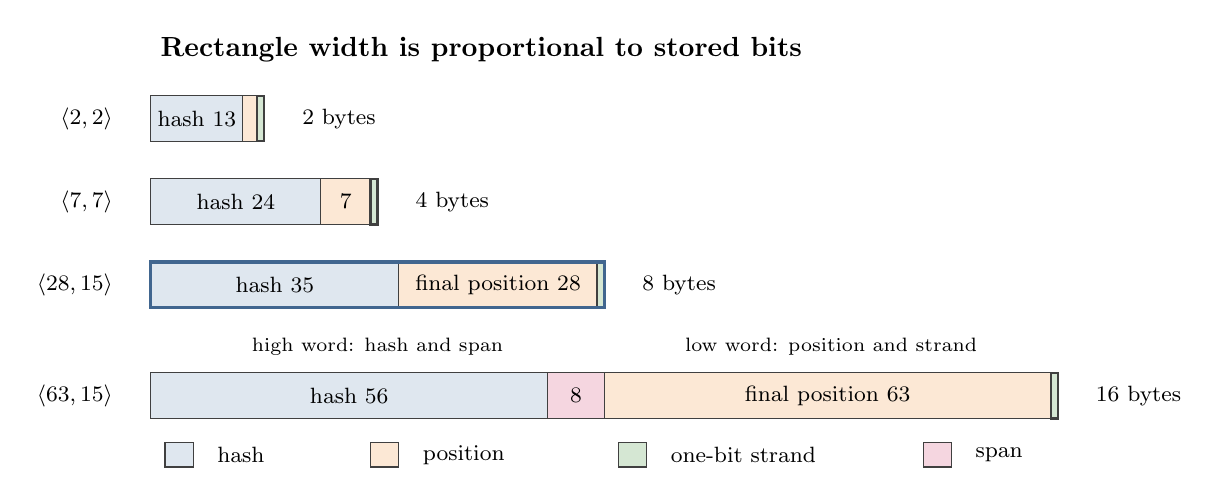
\begin{tikzpicture}[
  x=.09cm,
  y=.88cm,
  font=\footnotesize,
  hashfield/.style={draw=black!75,fill=rewriteBlue!18},
  posfield/.style={draw=black!75,fill=rewriteOrange!20},
  strandfield/.style={draw=black!75,fill=rewriteGreen!25},
  spanfield/.style={draw=black!75,fill=purple!16}
]
  \node[anchor=west,font=\bfseries] at (0,5.55)
    {Rectangle width is proportional to stored bits};

  \node[anchor=east] at (-4,4.55) {$\langle 2,2\rangle$};
  \draw[hashfield] (0,4.22) rectangle (13,4.88);
  \draw[posfield] (13,4.22) rectangle (15,4.88);
  \draw[strandfield,thick] (15,4.22) rectangle (16,4.88);
  \node at (6.5,4.55) {hash 13};
  \node[anchor=west] at (20,4.55) {2 bytes};

  \node[anchor=east] at (-4,3.35) {$\langle 7,7\rangle$};
  \draw[hashfield] (0,3.02) rectangle (24,3.68);
  \draw[posfield] (24,3.02) rectangle (31,3.68);
  \draw[strandfield,thick] (31,3.02) rectangle (32,3.68);
  \node at (12,3.35) {hash 24};
  \node at (27.5,3.35) {7};
  \node[anchor=west] at (36,3.35) {4 bytes};

  \node[anchor=east] at (-4,2.15) {$\langle 28,15\rangle$};
  \draw[hashfield] (0,1.82) rectangle (35,2.48);
  \draw[posfield] (35,1.82) rectangle (63,2.48);
  \draw[strandfield,thick] (63,1.82) rectangle (64,2.48);
  \draw[draw=rewriteBlue!85!black,very thick]
    (0,1.82) rectangle (64,2.48);
  \node at (17.5,2.15) {hash 35};
  \node at (49,2.15) {final position 28};
  \node[anchor=west] at (68,2.15) {8 bytes};

  \node[anchor=east] at (-4,.55) {$\langle 63,15\rangle$};
  \node[font=\scriptsize] at (32,1.25) {high word: hash and span};
  \node[font=\scriptsize] at (96,1.25) {low word: position and strand};
  \draw[hashfield] (0,.22) rectangle (56,.88);
  \draw[spanfield] (56,.22) rectangle (64,.88);
  \draw[posfield] (64,.22) rectangle (127,.88);
  \draw[strandfield,thick] (127,.22) rectangle (128,.88);
  \node at (28,.55) {hash 56};
  \node at (60,.55) {8};
  \node at (95.5,.55) {final position 63};
  \node[anchor=west] at (132,.55) {16 bytes};

  \draw[hashfield] (2,-.48) rectangle (6,-.13);
  \node[anchor=west] at (8,-.305) {hash};
  \draw[posfield] (31,-.48) rectangle (35,-.13);
  \node[anchor=west] at (37,-.305) {position};
  \draw[strandfield] (66,-.48) rectangle (70,-.13);
  \node[anchor=west] at (72,-.305) {one-bit strand};
  \draw[spanfield] (109,-.48) rectangle (113,-.13);
  \node[anchor=west] at (115,-.305) {span};
\end{tikzpicture}
\caption{Bit fields in four \texttt{minimizer\_representation<L,K>}
instantiations, shown from high bits on the left to low bits on the right.
Blue is the hash, orange is the zero-based final position, green is the
one-bit strand, and purple is the span in the two-word form.  The highlighted
$\langle28,15\rangle$ record is the default 64-bit sketch-data form.}
\label{fig:minimizer-representation-layout}
\end{figure}

The $L$-bit field represents final positions from zero through
$2^L-1$, so it can describe a local sequence span of at most $2^L$ bases.
For $K=15$, values through $L=33$ still fit in 64 bits, while $L=34$
requires the two-word form.  The $\langle28,15\rangle$ form has a 35-bit hash
field, but its minimap2 integer hash occupies only 30 bits.

Currently the main parameter that drives used representation width is the number of position bits $L$ (this is compared against \emph{kmer\_size\_buckets} array).
Theoretically the template can produce a two-byte record, but this bucket isn't suppored at this moment (such small width make's it problematic to adjust as we need to have very short hash, which isn't ideal as shorter k-mers are more prone to collisions or limit the size of sequence to less than 256, which would be very specific optimisation)
The $\langle2,2\rangle$ on the figure is just the demonstrative example to show that template is supported even in very degenerated edge cases (we don't actually use special form for sequences with less than 4 bases as it would make very little sense).


\section{Configured CPU algorithms}
\label{sec:configured-cpu-minimizers}

The PostgreSQL setting \texttt{bioseq.aligner.minimizer.algorithm} chooses the
minimizer implementation. Its current default is \texttt{bounded\_nthash\_simd}. Table~\ref{tab:current-cpu-minimizers}
maps the four CPU values to the algorithm families described earlier. Additionally we allow dispatching Vulkan kernel.

\begin{table}[H]
  \centering
  \small
  \begin{tabularx}{\linewidth}{@{}p{.37\linewidth}X@{}}
    \toprule
    \textbf{Setting value} & \textbf{Current CPU route} \\
    \midrule
    \texttt{scalar}
      & Scalar rescan with the minimap2 integer hash. \\
    \texttt{simd\_minimap2\_reference}
      & A1 with the minimap2 integer hash for DNA4 and a registered
        rank-based SIMD route for DNA5. \\
    \texttt{bounded\_nthash\_simd}
      & A2 with 32-bit ntHash for DNA4 and DNA5. A specialized
        $k=15,w=10$ kernel accompanies the generic runtime kernel. \\
    \texttt{two\_stack\_nthash}
      & Normally A3 chronological SIMD with the minimap2 integer hash. \\
    \bottomrule
  \end{tabularx}
  \caption{CPU minimizer implementations exposed by the PostgreSQL setting.}
  \label{tab:current-cpu-minimizers}
\end{table}

\info{Position locality}{
  In case of generating minimizers we can operate on local coordinates meaning that our minimizer representation can just track position relative to the sequence fragment. Sequence fragmentation in storage is described in later chapters.
  However for next steps of processing (chaining) we use global coordinates. It would be possible to take advantage of that locality for example by building index that stores only minimizers for some shorter sequence fragments (this is also described in later chapters), but for simplicity even in that case we just map local coordinates afterwards to global ones at all times.
  This have the cost of anchors being wider in memory (as we need to use int64 for global coordinates).
}




\flushbottom
